\documentclass{magnolia}

\magtex{tex_driver={pdftex},
        tex_packages={xypic}}
\magfiche{document_nom={Cours Python sur la complexité},
          auteur_nom={François Fayard},
          auteur_mail={fayard.prof@gmail.com}}
\magcours{cours_matiere={python},
          cours_niveau={mpsi},
          cours_chapitre_numero={7},
          cours_chapitre={Complexité}}
\magmisenpage{misenpage_presentation={tikzvelvia},
          misenpage_format={a4},
          misenpage_nbcolonnes={1},
          misenpage_preuve={non},
          misenpage_sol={oui}}
\maglieudiff{}
\magprocess

\begin{document}
%BEGIN_BOOK
\hfill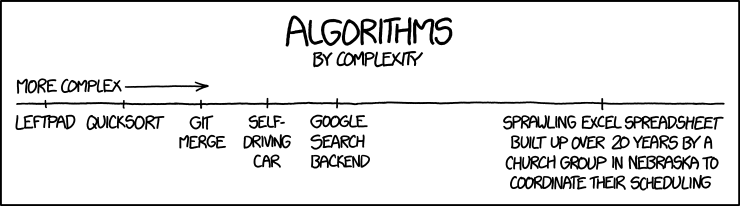
\includegraphics[width=0.6\textwidth]{../../Commun/Images/python-cours-algorithms}
\magtoc

\section{Complexité}
\subsection{Notation mathématique}

\begin{definition}
Soit $(u_n)$ et $(v_n)$ deux suites réelles positives
\begin{itemize}
  \item On dit que $u_n={\rm O}(v_n)$ lorsqu'il existe $B>0$ et $N\in\N$ tels que
    \[\forall n\geq N\qsep u_n \leq B v_n.\]
  \item On dit que $u_n=\Omega(v_n)$ lorsqu'il existe $A>0$ et $N\in\N$ tels que
    \[\forall n\geq N\qsep u_n \geq A v_n.\]
  \item On dit que $u_n=\Theta(v_n)$ lorsqu'il existe $A,B>0$ et $N\in\N$ tels que
    \[\forall n\geq N\qsep A v_n \leq u_n \leq B v_n.\]
\end{itemize}
\end{definition}

\begin{remarques}
\remarque On a $u_n=\Theta(v_n)$ si et seulement si  $u_n={\rm O}(v_n)$ et
  $u_n=\Omega(v_n)$.
\remarque La relation $\Theta$ est une relation d'équivalence sur l'ensemble des suites
  positives. En particulier, elle est symétrique.
\remarque Ces définitions sont asymptotiques~: Elles ne dépendent pas des premiers
  termes de ces suites.
\remarque Lorsque nous ferons des calculs de complexité, nous travaillerons avec des
  suites $(v_n)$ strictement positives. Dans ce cas
  \begin{itemize}
\item $u_n={\rm O}(v_n)$ si et seulement si il existe $B>0$ tel que~:
  $\forall n\in\N\qsep u_n\leq B v_n$.
\item $u_n=\Omega(v_n)$ si et seulement si il existe $A>0$ tel que~:
  $\forall n\in\N\qsep u_n \geq A v_n$.
\item $u_n=\Theta(v_n)$ si et seulement si il existe $A,B>0$ tels que~:
  $\forall n\in\N\qsep A v_n \leq u_n\leq B v_n$.
  \end{itemize}
  Ces caractérisations n'ont plus besoin du \og à partir d'un certain rang \fg.
\remarque Il faut bien retenir les interprétations intuitives~:
  \begin{itemize}
    \item \og $u_n = {\rm O}(v_n)$ \fg signifie \og $u_n$ est au plus de l'ordre de grandeur
de $v_n$ \fg.
    \item \og $u_n = \Omega(v_n)$ \fg signifie \og $u_n$ est au moins de l'ordre de grandeur
de $v_n$ \fg.
    \item \og $u_n = \Theta(v_n)$ \fg signifie \og $u_n$ et $v_n$ sont du même ordre de
grandeur \fg.
  \end{itemize}
\remarque Si $v_n=\Theta(w_n)$, alors une suite $u_n$ est un ${\rm O}$, un $\Omega$
  ou un $\Theta$ de $v_n$ si et seulement si c'est un ${\rm O}$, un $\Omega$ ou un
  $\Theta$ de $w_n$. En particulier, puisque quel que soit
  $b>1$, $\log_b n = \Theta(\ln n)$, dire que $u_n=\Theta(\log_2 n)$ est équivalent à dire que $u_n=\Theta(\ln n)$.
  On écrira simplement $u_n=\Theta(\log n)$.
\end{remarques}

\begin{proposition}
Soit $(u_n)$ une suite positive et $(v_n)$ une suite strictement positive. On suppose
que
\[\frac{u_n}{v_n} \tendvers{n}{+\infty} l\in\RP\cup\ens{+\infty}.\]
Alors
\begin{itemize}
\item $u_n={\rm O}(v_n)$ si et seulement si $l<+\infty$.
\item $u_n=\Omega(v_n)$ si et seulement si $l> 0$.
\item $u_n=\Theta(v_n)$ si et seulement si $0<l<+\infty$.
\end{itemize}
\end{proposition}

\begin{exoUnique}
\exo Déterminer les relations de comparaison entre les suites de terme général
  \begin{itemize}
    \item $u_n\defeq \ent{\ln n}$ et $v_n\defeq \ln n$.
    \item $u_n\defeq 12n^{2} + 3n\log n - n$ et $v_n\defeq n^{2}$.
    \item $u_n\defeq 12n^{2}$ et $v_n\defeq n^{17}$.
    \item $u_n\defeq 12n^{2}$ et $v_n\defeq n^{2}$.
    % \item $u_n\defeq  17 + (-1)^{n} + \frac{\ln n}{n}$ et $v_n\defeq 1$.
  \end{itemize}
\end{exoUnique}

\subsection{Type de ressource}

Étudier la complexité d'un algorithme, c'est s'intéresser aux ressources qu'il
consomme pour effectuer sa tâche, et plus précisément à la manière dont
cette consommation évolue lorsque la taille des données augmente. Les principales ressources auxquelles on peut s'intéresser sont~:
\begin{itemize}
  \item le \emph{temps} de calcul.
  \item l'\emph{espace} mémoire.
  \item l'\emph{énergie}, qui prend une importance de plus en plus grande
  à cause de son impact sur
  \begin{itemize}
  \item l'\emph{autonomie}, principalement dans les téléphones.
  \item le \emph{bilan écologique}
  et le \emph{cout monétaire} des calculs, principalement à l'échelle d'un
  datacenter.
  \end{itemize}
  \item les \emph{données échangées}  sur le réseau, qui peuvent être un facteur
  limitant.
\end{itemize}\medskip

% L'autre axe suivant lequel varie la notion de complexité est celui
% du niveau de détail souhaité. Tout d'abord, 
L'étude de la complexité se fait le plus souvent de manière
  \emph{asymptotique}, c'est-à-dire en faisant tendre la taille des données vers
  l'infini.
  
  \begin{definition}
On dit que la complexité $C(n)$ d'un algorithme est
\begin{itemize}
  \item \emph{constante} lorsque $C(n) = \Theta(1)$.
  \item \emph{logarithmique} lorsque $C(n)=\Theta(\log n)$.
  % \item \emph{poly-logarithmique} lorsque $f(n)=\Theta(P(\log n))$ où $P$ est un
  % polynôme de degré supérieur ou égal à $2$.
  \item \emph{linéaire} lorsque $C(n)=\Theta(n)$.
  \item \emph{quasi-linéaire} lorsque $C(n)=\Theta(n\log n)$.
  \item \emph{quadratique} lorsque $C(n)=\Theta\p{n^2}$.
  \item \emph{polynomiale} lorsqu'il existe $\alpha\in\N$ tel que $C(n)=\Theta\p{n^\alpha}$.
  \item \emph{exponentielle} lorsqu'il existe $\alpha>1$ tel que $C(n)=\Theta\p{\alpha^n}$.
  \item \emph{factorielle} lorsque $C(n)=\Theta\p{n!}$.
\end{itemize}
% On définit les mêmes notions pour la complexité en espace.
\end{definition}
  
% \begin{remarqueUnique}
%     \remarque
%   De nombreuses questions intéressantes en pratique ne rentrent pas
%   dans ce cadre, même si l'étude asymptotique peut orienter sur la bonne voie.
%   \begin{itemize}
%     \item Est-ce que je peux \emph{prouver} qu'il ne s'écoulera jamais plus de
%     50ms entre l'acquisition des données par les capteurs et l'envoi du signal
%     de commande aux actionneurs de mon nouvel avion ?
%     \item Est-ce que je vais arriver à produire en moyenne une image toutes les 16ms,
%     afin d'obtenir 60 images par seconde, sur un matériel précis ?
%     % \item Je reçois des transactions à traiter par paquets de mille, comment
%     % traiter un tel paquet le plus efficacement possible ?
%   \end{itemize}
%     \remarque
%   Même en se limitant à l'étude asymptotique, il reste beaucoup de variations.
%   \begin{itemize}
%     \item En théorie de la complexité, des questions typiques sont
%     \begin{itemize}
%       \item Cet algorithme est-il en temps polynomial ? De ce point de vue, le
%       tri rapide, le tri fusion et le tri par insertion se valent.
%       \item Cet algorithme est-il en temps élémentaire (c'est-à-dire majoré par
%       une tour d'exponentielles de hauteur bornée)~? Si la réponse est non, il
%       est temps de s'inquiéter.
%     \end{itemize}
%     \item Si l'on veut plus de détails, on peut simplement ignorer toutes les
%     constantes multiplicatives. On considère alors que toutes les opérations
%     élémentaires se valent (ajouter deux entiers machine, prendre le logarithme
%     d'un flottant, accéder à une case d'un tableau, etc), et on cherche
%     l'\emph{ordre de grandeur} du nombre total d'opérations effectuées en
%     fonction  de la taille $n$ des données. On dira alors que le tri fusion a
%     une complexité temporelle en $\Theta(n \log n)$ et le tri insertion en
%     $\Theta\left(n^2\right)$ dans le pire des cas.
%     \emph{C'est le point de vue du programme, et ce sera donc le nôtre.}
%     \item On peut bien sûr donner des résultats asymptotiques plus précis.
%     Typiquement, on comptera quelques types d'opérations élémentaires
%           et l'on cherchera un équivalent, voire mieux. Par exemple, on peut
%           prouver qu'en moyenne, sur une permutation aléatoire de $\interefo{0}{n}$,
%           le tri insertion effectue
%           \[\frac{n^{2}}{4} + \frac{3n}{4} - \ln n + {\rm O}(1)\]
%     comparaisons.
%   \end{itemize}
% \end{remarqueUnique}




% \section{Complexité en temps}

Quand on s'intéresse à la complexité temporelle d'un algorithme, on
cherche à évaluer comment son temps d'exécution évolue quand on
fait tendre la taille des données $n$ vers l'infini. Comme le temps
de calcul dépend de nombreux facteurs difficiles à contrôler
comme le langage, l'implémentation ou la machine,  on se concentre
sur le \emph{nombre d'instructions élémentaires} exécutées.
Il faut donc :
\begin{itemize}
  \item Déterminer le nombre de fois où
  chaque instruction est exécutée.
  \item Déterminer si chacune de ces instructions est \emph{élémentaire}
  ou non. Pour les instructions qui ne sont pas élémentaires, estimer leur
  complexité.
  \item Sommer toutes ces complexités et tenter éventuellement d'en tirer des conclusions sur le temps
  de calcul.
\end{itemize}

% Supposons pour l'instant que nous avons réussi à traiter le premier point,
% et intéressons-nous aux autres.

% \subsection{Opérations élémentaires en Python}
\vspace{2ex}
Ce qui caractérise une opération élémentaire, c'est qu'elle s'exécute
en temps constant. Dans l'idéal, il serait bon de ne considérer comme élémentaire
que les instructions assembleur exécutées par le processeur. En Python, les opérations
suivantes s'effectuent en temps constant~:
\begin{itemize}
  \item Utiliser les opérateurs \verb_not_, \verb!and!, et \verb!or! sur les booléens.
  \item Ajouter, soustraire, multiplier, diviser, comparer deux entiers ou deux flottants.
    Le fait que Python travaille avec des entiers de taille variable rend ces
    opérations non élémentaires, mais on supposera que les entiers que nous manipulons
    restent de taille raisonnable (disons qu'ils sont représentables sur 64~bits) ce
    qui a pour conséquence le fait que les opérations arithmétiques sur ces derniers restent
    élémentaires.
  \item Calculer la longueur d'une liste ou d'une chaine de caractères avec \verb!len(t)!, accéder à ou modifier
    l'élément d'indice $i$ d'une liste par \verb!t[i]!, accéder au caractère d'indice
    $i$ d'une chaine de caractères par \verb!s[i]!.
  \item Ajouter ou enlever un élément à la fin d'une liste grâce aux méthodes
    \verb_append_ et \verb_pop_.
  \item Enfiler ou défiler un élément sur une file du module \verb_collections_. Tester
    si une clé fait partie d'un dictionnaire, obtenir la valeur associée à une clé,
    créer, mettre à jour ou supprimer une association dans un dictionnaire.
  \item Affecter une variable.
  \item Appeler une fonction.
\end{itemize}
Cependant, les opérations suivantes ne s'effectuent pas en temps constant~:
\begin{itemize}
\item Si $x$ est un entier, le calcul de $x^n$ par \verb!x ** n! se fait en $\Theta(\log n)$.
\item La concaténation \verb!u + v! de deux chaines de caractères ou de deux listes
  $u$ et $v$ s'effectue en $\Theta(|u| + |v|)$.
\item La création d'une liste de taille $n$ par \verb![x] * n! s'effectue en
  $\Theta(n)$.
\item La méthode \verb!u.extend(v)! s'effectue en $\Theta(|v|)$.
\item Le slicing \verb!t[a:b:p]! s'effectue en un temps proportionnel à la longueur
  de la liste créée.
\end{itemize}

\vspace{2ex}
Dans de nombreux exemples, il arrive qu'on vous rappelle quelles sont les
opérations élémentaires que l'on doit prendre en compte pour le calcul de la complexité.
Par exemple, lors de l'étude de tris, il est courant de ne prendre en compte que le
nombre de comparaisons. Dans ce cas, les autres opérations doivent être ignorées.
Cependant, comme on détermine les complexités à un $\Theta$ près, la spécification exacte
des opérations élémentaires à prendre en compte n'a en général aucune influence sur le résultat final.


% Viennent s'ajouter deux fonctions essentielles à la gestion de le mémoire en C~: \verb!malloc! et \verb!free!.
% Malheureusement, la complexité de ces fonctions est très loin d'être simple~: elles ne peuvent même pas garantir
% leur exécution dans un temps fini. C'est pourquoi ces fonctions ne doivent pas être appelées dans le coeur de programmes dits
% temps réels, qui doivent garantir l'exécution dans un temps bien déterminé (matériel médical embarqué, logiciel de
% prise de décision dans un avion ou une voiture, logiciel de mixage musical, jeu vidéo). Cependant, elles utilisent
% des algorithmes qui font que dans la plupart des cas, elles répondent en temps constant. Sauf mention explicite du
% contraire, c'est cette hypothèse, qui est une simplification de la réalité, que nous ferons dans ce cours. La
% complexité des autres opérations de la bibliothèque standard ne sont en général pas en temps constant et seront données
% au cas par cas.\\

% En \textsc{OCaml}, certaines opérations du langage s'effectuent en temps constant alors d'autres ont une complexité
% plus élevée. Voici quelques exemples qu'il faut connaitre en \textsc{OCaml}.
% \begin{description}
%   \item[Opérations élémentaires] \
%   \begin{itemize}
%     \item Ajouter, soustraire, multiplier, diviser, comparer deux entiers machine ou deux flottants.
%     \item Créer une nouvelle liste \verb!hd :: tl! en ajoutant la tête \verb!hd! à une liste existante \verb!tl!.
%     \item Récupérer la tête et la queue d'une liste, en faisant un \verb!match!, ou en utilisant \verb!List.hd! et \verb!List.tl!.
%     \item Accéder à ou modifier l'élément \verb!i! d'un \verb!array! par \verb!t.(i)!.
%     \item Obtenir la longueur d'un \verb!array! par \verb!Array.length t!.
%   \end{itemize}
%   \item[Opérations non élémentaires] \
%   \begin{itemize}
%     \item Créer un tableau de taille $n$ à l'aide de \verb!Array.make n x!~: temps proportionnel à $n$.
%     \item Accéder à l'élément \verb!i! d'une liste~: temps proportionnel à \verb!i!.
%     \item Concaténer deux listes par \verb!u @ v!~: temps proportionnel à
%     $|\verb!u!|$.
%     \item Obtenir la longueur d'une liste par \verb!List.length u!~: temps
%     proportionnel à $|\verb!u!|$.
%   \end{itemize}
% \end{description}

% Pour plus de clareté, les sujets préciseront souvent les opérations qui seront considérées comme élémentaires.

% \subsection{Complexité}

\subsection{Complexité dans le pire des cas}

On donne toujours la complexité d'un algorithme en fonction de la
taille $n$ de l'entrée. Pourtant, la plupart des algorithmes peuvent
avoir un temps d'exécution très variable entre deux entrées de
même taille. 
La fonction suivante, qui cherche si un élément $x$ appartient ou
non à la liste $t$ de longueur $n$, s'exécute en temps
constant si le premier élément de $a$ vaut $x$, et en temps
proportionnel à $n$ si $x$ n'appartient pas à $t  $.

\begin{pythoncodeline}
def appartient(x, t):
    """appartient(x: int, t: list[int]) -> bool"""
    for i in range(len(t)):
        if t[i] == x:
            return True
    return False
\end{pythoncodeline}

% \begin{ccode}
% bool appartient(int x, int a[], int n) {
%     for (int i = 0; i < n; ++i) {
%         if (a[i] == x) {
%             return true;
%         }
%     }
%     return false;
% }
% \end{ccode}
\noindent
Par défaut, nous nous intéresserons toujours à la complexité
\emph{dans le pire des cas} : autrement dit, le $C(n)$ cherché
est le nombre maximum d'opérations élémentaires pour traiter une
entrée de taille $n$. Dans ce cadre, la fonction précédente a une complexité
en $\Theta(n)$.

\begin{definition}
Si un algorithme nécessite $C(d)$ opérations élémentaires pour s'exécuter
sur une donnée $d$, on appelle
\begin{itemize}
\item \emph{complexité dans le pire des cas} et on note $C_{\rm max}(n)$, le nombre maximal
  d'opérations élémentaires nécessaires pour traiter une donnée de taille
  $n$.
  \[C_{\rm max}(n)\defeq \max_{\abs{d}=n} C(d).\]
\item \emph{complexité dans le meilleur des cas} et on note $C_{\rm min}(n)$, le nombre minimal
  d'opérations élémentaires nécessaires pour traiter une donnée de taille
  $n$.
  \[C_{\rm min}(n)\defeq \min_{\abs{d}=n} C(d).\]
\end{itemize}
\end{definition}

\begin{exempleUnique}
\exemple Si on compte comme opération élémentaire le nombre de tests \verb!==!, la fonction \verb!appartient!
  a une complexité dans le pire et dans le meilleur des cas de
  \[C_{\rm max}(n)=n=\Theta(n), \qquad C_{\rm min}(n)=1=\Theta(1).\]
  Le pire cas est obtenu  lorsque le tableau ne contient pas l'élément $x$ et le meilleur des cas
  est obtenu lorsque l'élément $x$ est contenu dans la case d'indice 0 du tableau $t$.
\end{exempleUnique}

\subsection{Complexité en moyenne}

Certains algorithmes peuvent être très lents dans une petite
proportion de cas \og pathologiques \fg et très efficaces sur les autres.
Il peut alors être intéressant de calculer la \emph{complexité en moyenne}
de l'algorithme, c'est-à-dire l'espérance du temps de calcul
pour une certaine loi de probabilité sur les données. \smallskip

Ce type de complexité est plus délicat à étudier que la complexité
dans le pire des cas, et ce pour deux raisons.
\begin{itemize}
  \item Il n'est pas toujours évident de définir une loi de
  probabilité sur les données, et encore moins une loi de
  probabilité pertinente. Dans l'exemple précédent, quelle
  peut bien être la probabilité que le premier élément soit
  égal à $x$ ?
  \item Une fois que l'on a fixé la loi de probabilité, les
  calculs sont en général beaucoup plus délicats que pour le pire cas.
  Il peut même être nécessaire de faire des mathématiques très difficiles.
\end{itemize}

\begin{definition}
Si un algorithme nécessite $C(d)$ opérations élémentaires pour s'exécuter
sur une donnée $d$, et si $\mathbb{P}$ est une mesure de probabilité
sur l'ensemble des données de taille $n$, on appelle \emph{complexité en moyenne} et on note $C_{\rm moy}(n)$
le nombre
\[C_{\rm moy}(n)\defeq \sum_{\abs{d}=n} \mathbb{P}(d) C(d)\]
\end{definition}

\begin{remarques}
\remarque Dans le cas où il existe un nombre fini $m$ de données $d_1,\ldots,d_m$ de taille $n$, on prend
  le plus souvent la loi de probabilité uniforme. Dans ce cas
  \[C_{\rm moy}(n)\defeq \frac{1}{m}\sum_{k=1}^m C(d_k).\]
\remarque On a bien évidemment
  \[C_{\rm moy}(n) = {\rm O}(C_{\rm max}(n)) \quad\text{et}\quad C_{\rm moy}(n) = \Omega(C_{\rm min}(n)).\]
\remarque L'exemple le plus connu, et sans doute le plus important, d'algorithme
pour lequel il est pertinent de faire une analyse en moyenne est
celui du \emph{tri rapide}. En effet, il est en $\Theta\left(n^2\right)$
dans le pire des cas mais en $\Theta(n \log n)$ en moyenne si
le tableau d'entrée est dans un ordre aléatoire. De plus, étant donné qu'il se fait
en place, il est
souvent plus efficace que le tri fusion qui est pourtant en
$\Theta(n \log n)$ dans le pire cas.
\remarque Voici les complexités des différents algorithmes de tri que nous avons vu~:
\begin{center}
\begin{tabular}{|l|c|c|c|}
\hline
Méthode & $C_{\rm min}(n)$ & $C_{\rm moy}(n)$ & $C_{\rm max}(n)$ \\
\hline
\hline
Tri sélection & $\Theta\p{n^2}$ & $\Theta\p{n^2}$& $\Theta\p{n^2}$\\
\hline
Tri insertion & $\Theta\p{n}$& $\Theta\p{n^2}$& $\Theta\p{n^2}$\\
\hline
Tri fusion & $\Theta\p{n \log n}$ & $\Theta\p{n \log n}$& $\Theta\p{n \log n}$\\
\hline
Tri rapide & $\Theta\p{n \log n}$& $\Theta\p{n \log n}$&  $\Theta\p{n^2}$\\
\hline
\end{tabular}
\end{center}
\end{remarques}

% \subsection{Complexité amortie}

% Nous avons vu dans le TP sur les tableaux dynamiques la réalisation d'une structure
% de donnée mutable linéaire permettant~:
% \begin{itemize}
% \item Un accès au $k$-ième élément en $\Theta(1)$.
% \item Une opération appelée \verb!append! (ou parfois \verb!push!) ajoutant l'élément $x$ à la fin de la structure.
% \item Une opération appelée \verb!pop! renvoyant le dernier élément de la structure et enlevant cet élément.
% \end{itemize}
% Cette structure de donnée est fondamentale en programmation impérative et elle est disponible en Python
% sous le nom (très mal choisi) de liste et en C++ sous le nom de \verb!std::vector!. Elle n'est malheureusement
% pas disponible dans la bibliothèque standard de \textsc{OCaml}.\\

% Nous avons vu que si nous appelons \verb!append! sur un tableau de longueur $n$, même dans l'implémentation
% optimisée utilisant un tableau ayant une taille $n$ et une capacité $p$, lorsque $n=p$ une nouvelle
% allocation mémoire est nécessaire pour créer un tableau de taille $2n$ et une recopie de l'ancien tableau est nécessaire.
% La complexité dans le pire des cas de la fonction \verb!append! est donc en $\Theta(n)$. Cependant, on montre que
% si l'on part d'une liste vide, $n$ appels à la fonction \verb!append! nécessitent dans le pire des cas $\Theta(n)$
% opérations. En moyenne, la fonction \verb!append! nécessite donc $\Theta(1)$ opérations. On dit dans ce cas que la
% \emph{complexité amortie} de la fonction append est en $\Theta(1)$. Cette notion de complexité amortie est souvent pertinente
% pour l'analyse des structures de données.

\subsection{Complexité temporelle et temps de calcul}

Après avoir analysé la complexité temporelle d'un algorithme, on dispose
d'une information du type $T(n) = \Theta(n \log n)$.
En théorie, cela ne nous dit absolument rien du temps de calcul réel pour
une valeur donnée de $n$, mais en pratique on peut en tirer
quelques informations.\\

\emph{Valeur de la constante cachée}~: Pour un algorithme raisonnablement
simple, on peut supposer que la constante multiplicative cachée dans le
$\Theta$ est de l'ordre de 10, voire de 100. Pour certains algorithmes
très sophistiqués, elle peut cependant être très grande et rendre l'algorithme
beaucoup moins efficace qu'on ne le pense, voire inutilisable en pratique.\\

\emph{Traduction d'une opération élémentaire}~: Certaines des opérations
élémentaires vues plus haut (ajouter deux flottants, par exemple)
correspondent directement à une instruction processeur. D'autres sont plus
complexes et correspondront à plusieurs instructions (une bonne centaine pour faire un
\verb!append! en Python).\\

\emph{Cycle processeur}~: Vu de l'extérieur, l'état d'un processeur évolue
de manière discrète. Il est dans un certain état à l'instant $t_n$, dans un
certain état à l'instant $t_{n + 1} = t_n + h$ et dans un état non défini entre
ces deux instants. Ce $h$ est la durée d'un \emph{cycle}, c'est-à-dire l'inverse
de la \emph{fréquence d'horloge} que les constructeurs communiquent. Comme vous
le savez peut-être, la fréquence d'un processeur actuel varie entre $1~{\rm GHz}$ et
$5~{\rm GHz}$, et un cycle prend donc de $0.2{\rm ns}$ à $1{\rm ns}$.\\


\emph{Temps pour exécuter une instruction}~: Exécuter une instruction prend
au moins un cycle (un processeur peut cependant exécuter plusieurs
  instructions en parallèle sur un même cœur), mais peut prendre
beaucoup plus longtemps. Quelques exemples~:
\begin{itemize}
  \item Ajouter deux entiers, comparer deux flottants : 1 cycle.
  \item Une division entière : Une vingtaine de cycles.
  \item Le calcul du cosinus d'un nombre flottant : Une centaine de cycles.
  \item Accès mémoire : entre 1 et 1000 cycles.
\end{itemize}
\vspace{2ex}

\noindent
\emph{Une recette de cuisine}~: En étant optimiste
\begin{itemize}
  \item La constante cachée vaut 2 (très optimiste).
  \item Chaque opération élémentaire donne 5 instructions (optimiste).
  \item On a un IPC (nombre d'instructions exécutées par cycle d'horloge) de 2 (très raisonnable).
  \item Un cycle prend $0.2{\rm ns}$ (optimiste).
\end{itemize}
On arrive alors à un temps de calcul de $f(n)$ nanosecondes si la complexité est
en $\Theta(f(n))$. C'est possible si par exemple on programme bien une
multiplication matricielle en assembleur, voire en C.
Si au contraire on travaille dans un langage \og lent \fg comme Python et si
l'algorithme se prête moins à un traitement efficace en machine, on peut
facilement être mille fois plus lent. On pourra donc retenir la recette
suivante~: \emph{Si la complexité temporelle est en $\Theta(f(n))$,
pour des valeurs de $n$ \og pas trop petites \fg, le temps de
  calcul sera le plus souvent compris entre $f(n)$ nanosecondes et
  $f(n)$ microsecondes}.


% \begin{figure}[H]
%   \centering
\begin{center}
  \begin{tabular}{>{\bfseries}c*6{c}}
    \toprule
                       & 10      & 100    & \nombre{1\ 000} & \nombre{10\ 000} & \nombre{1\ 000\ 000} & $10^9$  \\
    \otoprule
    $\Theta(\log n)$   & 1{\rm ns}    & 10{\rm ns}  & 10{\rm ns}  & 10{\rm ns} & 10{\rm ns} & 100{\rm ns}  \\
    \midrule
    $\Theta(\sqrt{n})$ & 1{\rm ns}    & 10{\rm ns}  & 100{\rm ns} & 100{\rm ns} & 1{\rm mics} & 1{\rm ms} \\
    \midrule
    $\Theta(n)$        & 10{\rm ns}   & 100{\rm ns} & 1{\rm mics} & 10{\rm mics} & 1{\rm ms} & 1{\rm s} \\
    \midrule
    $\Theta(n\log n)$  & 10{\rm ns}   & 100{\rm ns} & 10{\rm mics} & 100{\rm mics} & 10{\rm ms} & 10{\rm s} \\
    \midrule
    $\Theta(n^2)$      & 100{\rm ns}  & 10{\rm mics} & 1{\rm ms} & 100{\rm ms} & 10 min & 10 ans \\
    \midrule
    $\Theta(n^3)$      & 1{\rm mics}  & 1{\rm ms}   & 1{\rm s} & 10 min & 10 ans & $\infty$ \\
    \midrule
    $\Theta(2^n)$      & 1{\rm mics}  & $\infty$ & $\infty$ & $\infty$ & $\infty$ & $\infty$ \\
    \bottomrule
  \end{tabular}\\
  \vspace{2ex}
  Ordre de grandeur du temps de calcul pour quelques valeurs de $n$ et complexités
    usuelles.
\end{center}
\noindent
 On est ici très optimiste : il faut par exemple comprendre que pour une
 complexité en $\Theta(n\log n)$ avec $n = 10^6$, on prendra \emph{au mieux quelques dizaines
   de millisecondes}. Pour une version pessimiste, il faut essentiellement tout
 multiplier par mille.

% \subsubsection{Quelques résultats expérimentaux}

% \paragraph*{Tri rapide en \textsc{OCaml}}

% Le tri rapide est un algorithme de tri qui a une complexité de $\Theta(n \log n)$ en moyenne si le tableau
% à trier est aléatoire. En prenant une implémentation raisonnablement
% efficace de cet algorithme en \textsc{OCaml}, on obtient pour un tableau de
% un million d'éléments :
% \begin{description}
%   \item[Nombre d'instructions~:] Environ 450 millions, donc le $A$ de $An\log n$
%   vaut à peu près 20.
%   \item[Instructions par cycle~:] environ 1.3.
%   \item[Durée d'un cycle~:] Environ 0.3{\rm ns} \ (ne dépend que de l'ordinateur).
%   \item[Temps d'exécution~:] Environ 100{\rm ms}\ (pourrait se déduire des trois points
%   précédents).
% \end{description}
% Sachant que $n\log n$ vaut environ 20 millions pour $n = 10^6$, la
% \og recette de cuisine \fg prédisait entre 20 millisecondes et 20 secondes :
% on est dans la partie basse de la fourchette.\\

% Les graphiques ci-dessous permettent de visualiser ce qui se passe pour
% différentes valeurs de $n$ : le nombre d'instructions est toujours
% d'environ $20n\log n$.

% % \begin{figure}[H]
% %   \centering
% %   \begin{multicols}{2}
%     \begin{center}
%     \includegraphics[width = 8.5cm]{../../Commun/Images/info-cours-rapide-temps.pdf}
%     % \hspace{2cm}
%     \includegraphics[width = 8.5cm]{../../Commun/Images/info-cours-rapide-instr-nlogn.pdf}\\
%  Tri rapide en \textsc{OCaml} (raisonnablement optimisé).
%     \end{center}
%   % \end{multicols}
% % \end{figure}

% \paragraph*{Dichotomie en \textsc{OCaml}}

% Pour la recherche dichotomique dans un tableau trié, on trouve
% bien un nombre d'instructions en $A\log n$ avec $A \simeq 20$,
% mais le nombre d'instructions par cycle varie significativement
% avec $n$ (quand le tableau devient trop grand, il ne tient plus
% dans le \emph{cache}, qui est plus ou moins la partie \og rapide \fg
% de la mémoire).

% % \begin{multicols}{2}
% %   \begin{figure}[H]
% %     \centering
% \begin{center}
%     \includegraphics[width = 10.4cm]{../../Commun/Images/info-cours-dicho-ocaml-instructions}\\
%     Le nombre d'instructions par recherche vaut environ $20\log n$.
% \end{center}
%   % \end{figure}

%   % \begin{figure}[H]
%   %   \centering
%   \begin{center}
%     \includegraphics[width = 10.4cm]{../../Commun/Images/info-cours-dicho-ocaml-ipc}\\
%     Le nombre d'instructions par cycle décroît fortement avec $n$.\\
%     Cela est dû au fait que le tableau ne tient plus dans le cache.
%   \end{center}
% %   \end{figure}
% % \end{multicols}

% % \begin{figure}[H]
% %   \centering
% \begin{center}
%   \includegraphics[width = 11cm]{../../Commun/Images/info-cours-dicho-ocaml-temps}\\
%   Si le temps par recherche était proportionnel à $\log n$, on
%     obtiendrait une droite.
% \end{center}
% % \end{figure}

% \newpage

% \paragraph*{Tri insertion en \textsc{OCaml} et tri fusion en Python}~:
% Pour observer l'impact relatif des constantes multiplicatives
% et des complexités asymptotiques, on peut comparer un tri
% insertion bien écrit en \textsc{OCaml} et un tri fusion très naïf en Python,
% c'est-à-dire un algorithme en $An^2$ et un en $Bn\log n$ avec
% $A \ll B$.
% % \begin{multicols}{2}
% %   \begin{figure}[H]
% %     \centering
%     \begin{center}
%     \includegraphics[width = 10.5cm]{../../Commun/Images/info-cours-fusion-python-instr-nlogn}\\
%     Le nombre d'instructions exécutées par cette variante du
%     tri fusion\\ en Python est de l'ordre de $3\ 000\ n\log n$.
%     \end{center}
%   % \end{figure}

%   % \begin{figure}[H]
%   %   \centering
%     \begin{center}
%     \includegraphics[width = 10.5cm]{../../Commun/Images/info-cours-comparaison-temps}\\
%     Comparaison de temps de calcul\\
%     La courbe rouge est le temps de calcul pour un tri rapide en OCaml.
%     \end{center}
% %   \end{figure}
% % \end{multicols}



\section{Calcul de complexité temporelle}

Dans cette partie, on suppose que l'on connait la complexité de toutes
les fonctions prédéfinies qu'on utilise (on sait donc que \verb!len!
est en $\Theta(1)$  par
exemple), et que l'on souhaite calculer la complexité temporelle dans
le pire cas d'une fonction. Autrement dit, on cherche une estimation asymptotique
du nombre $C(n)$ d'opérations effectuées dans le pire cas, idéalement sous
la forme d'un $\Theta$, ou d'un \og bon \fg O. Si nous parlons d'un
bon \og O\fg , c'est que si 
  vous prouvez rigoureusement que
  la complexité du tri par insertion est en ${\rm O}(n!)$, vous n'avez
  certes pas commis d'erreur, mais vous n'avez pas non plus obtenu de points.

\subsection{Algorithme itératif}

\subsubsection{Boucles for}

Pour une boucle \verb_for_, il faut simplement sommer le nombre d'opérations pour chacune des
itérations.\\

Commençons par l'exemple du tri par sélection, dont le code nous est rappelé ci-dessous~:
\begin{pythoncodeline}
def swap(t, i, j):
    """swap(t: list[int], i: int, j: int) -> NoneType"""
    t[i], t[j] = t[j], t[i]

def indice_minimum(t, i):
    """indice_minimum(t: list[int], i: int) -> int"""
    j_min = i
    for j in range(i + 1, len(t)):
        if t[j] < t[j_min]:
            j_min = j
    return j_min

def tri_selection(t):
    """tri_selection(t: list[int]) -> NoneType"""
    for i in range(len(t) - 1):
        j = indice_minimum(t, i)
        swap(t, i, j)
\end{pythoncodeline}
La fonction \verb!swap! s'effectue en $\Theta(1)$ car elle n'effectue que deux accès
mémoire et deux affectations. Si on note $n$ la longueur du tableau, la fonction
\verb!indice_minimum! effectue quant à elle $n-1-i$ passages dans la boucle. Comme
les opérations à l'intérieur de la boucle sont élémentaires, sa complexité est donc
en $\Theta(n-1-i)$. La complexité de la fonction \verb!tri_selection! est donc en
\begin{eqnarray*}
C(n)=\sum_{i=0}^{n-2} \cro{\Theta(n-1-i) + \Theta(1)}
&=& \sum_{i=0}^{n-2} \Theta(n-1-i) = \Theta\p{\sum_{i=0}^{n-2} (n-1-i)}\\
&=& \Theta((n-1)+\cdots+2+1) = \Theta\p{\frac{n(n-1)}{2}}\\
&=& \Theta(n^2).
\end{eqnarray*}
L'algorithme de tri sélection est donc un algorithme de complexité quadratique.
Remarquons que nous aurions trouvé le même résultat si nous avions seulement
compté le nombre de comparaisons.\\

Attention à bien voir la différence entre des boucles
  \emph{successives} qui donnent une complexité en $\Theta(n)$ si les corps
  de boucle sont des instructions élémentaires
\begin{pythoncodeline}
for i in range(n):
    (*@\textcolor{purple}{corps de................}@*)  # On passe n fois ici
    (*@\textcolor{purple}{..................boucle}@*)
for i in range(n):
    (*@\textcolor{purple}{corps de................}@*)  # On passe n fois ici
    (*@\textcolor{purple}{..................boucle}@*)
\end{pythoncodeline}
et des boucles \emph{imbriquées} qui donnent une complexité en $\Theta(n^2)$ dans
la même situation.
\begin{pythoncodeline}
for i in range(n):
    for j in range(n):
        (*@\textcolor{purple}{corps de................}@*)  # On passe n^2 fois ici
        (*@\textcolor{purple}{..................boucle}@*)
\end{pythoncodeline}

% \begin{remarqueUnique}
%   % \remarque Il faut faire bien attention à ne pas multiplier des complexités alors qu'on
%   % devrait les ajouter. Essentiellement, on fait toujours des sommes de
%   % complexité, qui peuvent éventuellement se transformer en produits quand
%   % tous les termes sommés sont égaux, par exemple dans le cas où $f$ est
%   % en $\Theta(n)$.
%   % En particulier, si vous obtenez une complexité en $n!$, vous avez
%   % \emph{presque certainement fait une erreur} en remplaçant un
%   % $\sum_{i = 1}^n i$ par un $\prod_{i = 1}^n i$.
%   \remarque 
% \end{remarqueUnique}
\vspace{2ex}
Prenons désormais un exemple un peu plus général. 
On suppose maintenant que $f$ est une fonction
de signature \verb!f(t: list[int], i: int) -> int!, et on considère la fonction~:

\begin{pythoncodeline}  
def g(t):
    """g(t: list[int]) -> NoneType"""
    n = len(t)
    for i in range(n):
        j = f(t, i)
        t[i] = j
\end{pythoncodeline}

% \begin{camlcode}
% let exemple (t : int array) =
%   let n = Array.length t in
%   let f i = ... in
%   for i = 0 to n - 1 do
%     let x = f i in
%     t.(i) <- x + i
%   done
% \end{camlcode}
\noindent
La ligne 3 n'est exécutée qu'une seule fois, et prend un temps unitaire.
Les lignes 5 et 6, le \emph{corps} de la boucle, sont exécutées $n$ fois
chacune. La ligne 6 est une opération élémentaire, mais la ligne 5 contient
un appel à une fonction inconnue $f$ avec le paramètre $i$. Le nombre
total d'instructions exécutées dans cette boucle est donc
\[C(n)=\sum_{i = 0}^{n - 1} \cro{1 + T(i)}.\] où $T(i)$ correspond au
nombre d'instructions pour le calcul de \verb!f(t, i)!.

\begin{itemize}
  \item Si $f$ s'exécute en temps constant,
  par exemple si
\begin{pythoncodeline}
def f(t, i):
    """f(t: list[int], i: int) -> int"""
    return t[i]
\end{pythoncodeline}
  alors chaque itération est en
  $\Theta(1)$ et on obtient au total
  \[C(n)=\sum_{i=0}^{n-1} \cro{1+\Theta(1)}=\sum_{i=0}^{n-1} \Theta(1)=\Theta(n).\]
  \item Le temps d'exécution de \verb!f(t, i)! pourrait aussi dépendre de \verb!n!,
  tout en restant indépendant de \verb!i!. Par exemple
\begin{pythoncodeline}
def f(t, i):
    """f(t: list[int], i: int) -> int"""
    k = 0
    n = len(t)
    for j in range(n):
        if t[j] < t[i]:
            k += 1
    return k
\end{pythoncodeline}
  Dans ce cas, chacun des termes de la somme  est un $\Theta(n)$,
  et l'on obtient donc
  \[C(n)=\sum_{i = 0}^{n - 1} \cro{1 + \Theta(n)}
        =\sum_{i = 0}^{n - 1} \Theta(n)
        =\Theta\p{\sum_{i=0}^{n-1} n}=\Theta\p{n^2}.\]
  \item Considérons maintenant la fonction \verb!f! suivante, qui s'exécute en
  temps $\Theta(i)$.
\begin{pythoncodeline}
def f(t, i):
    """f(t: list[int], i: int) -> int"""
    k = 0
    for j in range(i):
        if t[j] < t[i]:
            k += 1
    return k
\end{pythoncodeline}
  \begin{itemize}
    \item Le calcul de la complexité totale ne pose pas de problème
    \[
     C(n)=\sum_{i = 0}^{n - 1} \cro{1+\Theta(i)}
         =\sum_{i = 0}^{n - 1} \Theta(i)
         =\Theta\p{\sum_{i = 0}^{n - 1} i}
         =\Theta\left(\frac{n(n - 1)}{2}\right)
         =\Theta(n^2).
    \]

    \item Comme on a toujours $i < n$, la fonction $f$ s'exécute en temps
    ${\rm O}(n)$. Si l'on souhaite seulement une \emph{majoration} de la
    complexité totale, on peut donc écrire
    \[
      C(n)=\sum_{i = 0}^{n - 1} \cro{1+{\rm O}(n)}
      =\sum_{i = 0}^{n - 1} {\rm O}(n)
      ={\rm O}\p{\sum_{i = 0}^{n - 1} n}
      = {\rm O}(n^2).
    \]
    Au point précédent, on avait obtenu une estimation plus précise : notre \og~grand-O~\fg est en fait
    un $\Theta$.
Ce ne sera pas toujours le cas. Par exemple, si la fonction $f$
  s'exécute en temps $\Theta(2^i)$, alors une majoration brutale donnerait
  \[
    C(n)=\sum_{i = 0}^{n - 1} \cro{1+\Theta\p{2^i}}
    =\sum_{i = 0}^{n - 1} \Theta\p{2^i}
    =\sum_{i = 0}^{n - 1} {\rm O}\p{2^n}
    ={\rm O}\p{\sum_{i = 0}^{n - 1} 2^n}
    = {\rm O}(n2^n).
  \]
  C'est correct, car c'est bien une \emph{majoration}, mais elle est grossière. En
  réalité, on a
  \[
    C(n)
    =\sum_{i = 0}^{n - 1} \Theta\p{2^i}
    =\Theta\p{\sum_{i=0}^{n-1} 2^i}
    =\Theta(2^n - 1)
    = \Theta(2^n).
  \]
\end{itemize}
\end{itemize}

Dans les exemples précédents, nous avons à plusieurs reprises dû trouver un ordre
de grandeur de la somme $\sum_{k=0}^{n-1} k$. Comme nous sommes amenés à 
manipuler des sommes de ce type, on pourra utiliser directement les résultats suivants~:


\begin{proposition}
  Soit $\alpha,\beta\geq 0$ et $\gamma>1$. Alors
\[\sum_{k=0}^n k^\alpha = \Theta(n^{\alpha+1}), \qquad
  \sum_{k=1}^n k^\alpha \log^\beta k  = \Theta(n^{\alpha+1}\ln^\beta n)
  \quad\et\quad \sum_{k=0}^n \gamma^k = \Theta(\gamma^n).\]
\end{proposition}

\subsubsection{Boucle while}

La différence avec une boucle \verb!for! est qu'on ne connait pas
\emph{à priori} le nombre d'itérations. Le plus souvent, on sera amené
à le majorer, mais il faudra faire attention à ne pas être trop grossier.\\


%   On considère les deux fonctions suivantes, et l'on note $n = |t|$.
% \begin{pythoncode}
% def nb_zeros(t, i):
%     """nb_zeros(t: list[int], i: int) -> int"""
%     j = 0
%     n = len(t)
%     while i + j < n and t[i + j] == 0:
%         j += 1
%     return j
% \end{pythoncode}

% \begin{pythoncode}
% def bloc_max_zeros(t):
%     """bloc_max_zeros(t: list[int]) -> int"""
%     m = 0
%     i = 0
%     n = len(t)
%     while i < n:
%         j = nb_zeros(t, i)
%         m = max(m, j)
%         i = i + j + 1
%     return m
% \end{pythoncode}
%   \begin{itemize}
%     \item $\ $Pour la fonction \verb!nb_zeros!, la condition et le corps de la boucle sont
%     en ${\rm O}(1)$, et l'on fait au plus $n - i$ itérations, donc la complexité est
%     en ${\rm O}(n - i)$. Le nombre exact d'itérations dépend de la position du premier
%     zéro, mais notre majoration est optimale dans le pire des cas.
%     \item $\ $Pour la fonction \verb!bloc_max_zeros!, la complexité de chaque itération
%     est dominée par celle de l'appel à \verb!nb_zeros!. Comme \verb!i! augmente d'au moins
%     un à chaque itération, on peut majorer grossièrement et obtenir pour la
%     complexité totale :
%     \[
%       \sum_{i = 0}^{n - 1} {\rm O}(n - i) = {\rm O}\p{n^2}
%     \]
%     C'est \emph{correct}, mais bien trop \emph{imprécis} !
%     \item $\ $En réalité, le temps d'exécution de \verb|nb_zeros(t, i)| est proportionnel
%     à la valeur renvoyée. Ainsi, en notant $0 = i_0,\dots,i_p=n$ les valeurs
%     successives de \verb!i!, la $k$-ème itération prend un temps proportionnel
%     à $i_k - i_{k - 1}$. Au total, on obtient donc
%     \[
%       \sum_{k = 1}^p {\rm O}(i_k - i_{k - 1})
%       = {\rm O}(i_p - i_0) = {\rm O}(n).
%     \]
%     \item $\ $En pratique, on rédigerait de manière moins formelle : \verb|nb_zeros(t, i)|
%     parcourt un morceau de \verb!t! de taille \verb!j! en temps ${\rm O}(j)$, et la ligne
%     \verb|i = i + j + 1| assure qu'on ne parcourt jamais deux fois la même case.
%     Au total, on effectue donc un unique parcours de \verb!t!, en temps
%     ${\rm \Theta}(n)$.
%   \end{itemize}

Revenons à l'exemple de la recherche d'un élément d'une liste triée par dichotomie, dont
nous avons donné le code dans le chapitre sur les listes.
\begin{pythoncodeline}
def dichotomie(x, t):
    """dichotomie(x: int, t: list[int]) -> bool"""
    g = 0
    d = len(t)
    while g < d:
        m = (g + d) // 2
        if x == t[m]:
            return True
        elif x < t[m]:
            d = m
        else:              # Cas où x > t[m]
            g = m + 1
    return False
\end{pythoncodeline}
On note $g_k$ et $d_k$ les valeurs respectives de \verb!g! et \verb!d! lors du passage
d'indice $k$ dans la boucle. On a $g_0\defeq 0$ et $d_0\defeq n$ et, dans les
deux cas où $x$ n'est pas trouvé à l'itération $k$, on montre que
\[d_{k+1}-g_{k+1}\leq \frac{d_k-g_k}{2}\]
Autrement dit, la largeur $l_k\defeq d_k-g_k$ de la tranche de recherche est
au moins divisée par
2 à chaque itération. On en déduit que
\[l_k \leq \frac{n}{2^k}.\]
Dès que $l_k\leq 1$, on sort de la boucle au plus tard à l'itération suivante. Or
\[\frac{n}{2^k} \leq 1 \quad\ssi\quad 2^k\geq n \quad\ssi\quad \log_2(2^k) \geq \log_2 n
  \quad\ssi\quad k \geq \log_2 n \quad\ssi\quad k\geq \ents{\log_2 n}.\]
Cet algorithme effectue donc au plus $1+\ents{\log_2 n}$ itérations.
La complexité dans le pire des cas de la recherche dichotomique
est donc en ${\rm O}(\log n)$. Comme ces itérations sont toutes effectuées si la liste
ne contient pas l'élément recherché, on se convaincra que cette complexité est 
en fait en $\Theta(\log n)$. D'autre part, la complexité dans le meilleur
des cas est en $\Theta(1)$, ce cas étant atteint lorsque l'élément $x$ est exactement
au milieu de notre liste.\\

\begin{remarqueUnique}
\remarque
  Attention, il ne faut pas oublier de prendre en compte le
  temps nécessaire à évaluer la condition de la boucle. Pour prendre
  un exemple un peu idiot, la fonction suivante s'exécute
  en temps $\Theta(|u|^2)$.
\begin{pythoncodeline}
def somme(t):
    """somme(t: list[int]) -> int"""
    s = 0
    for x in t:
        s = s + x
    return s

def f(u, borne):
    """f(u: list[int], borne: int) -> int"""
    i = 0
    while i < len(u) and somme(u[:i]) < borne: # Evaluation en O(i) !!!
        i += 1                                 # Corps de la boucle en O(1)
    return i
\end{pythoncodeline}
\end{remarqueUnique}

\subsection{Algorithme récursif}

Pour la complexité temporelle, les algorithmes récursifs font naturellement apparaitre
une formule de récurrence. Diverses techniques que nous allons voir nous permettent
d'en déduire le comportement asymptotique.\\

Dans les cas les plus simples, on commencera par établir une forme close pour $C(n)$.
Prenons l'exemple de la fonction suivante qui calcule la factorielle d'un entier
positif~:
\begin{pythoncodeline}
def factorielle(n):
    """factorielle(n: int) -> int"""
    if n == 0:
        return 1
    else:
        return n * factorielle(n - 1)
\end{pythoncodeline}
On souhaite estimer la complexité de cette fonction en calculant le nombre $C(n)$ de
multiplications effectuées. La lecture du code nous donne
\[C(0)=0, \quad\et\quad \forall n\in\Ns\qsep C(n)=C(n-1)+1.\]
On en déduit que $C(n)=n$ et donc que $C(n)=\Theta(n)$.\\

Mais rapidement, on se rend compte que les formes closes pour $C(n)$ deviennent complexes.
Considérons par exemple l'algorithme d'exponentiation rapide dans sa version récursive~:
\begin{pythoncodeline}
def expo_rapide(x, n):
    """expo_rapide(x: int, n: int) -> int"""
    if n == 0:
        return 1
    else:
        p = n // 2
        y = expo_rapide(x, p)
        if n % 2 == 0:
            return y * y
        else:
            return x * y * y
\end{pythoncodeline}
Si on note $C(n)$ le nombre de multiplications effectuées pour le calcul de $x^n$, on a
\[C(0)=0\qsep\text{et}\quad \forall n\in\Ns\qsep C(n)=
  \begin{cases}
  C(\ent{n/2}) + 1 & \text{Si $n$ est pair,}\\
  C(\ent{n/2}) + 2 & \text{Si $n$ est impair.}
  \end{cases}\]
Cette récurrence devient plus facile à appréhender si l'on décompose $n$ en
base 2. Si $n=\underline{d_{w-1}\ldots d_1 d_0}_2$, on a
\[C(\underline{d_{w-1}\ldots d_1 d_0}_2)=
  \begin{cases}
  C(\underline{d_{w-1}\ldots d_1}_2) + 1 & \text{Si $d_0=0$,}\\
  C(\underline{d_{w-1}\ldots d_1}_2) + 2 & \text{Si $d_0=1$.}
  \end{cases}\]
En notant $z(n)$ le nombre de 0 dans la décomposition de $n$ en base 2 et $u(n)$ le nombre
de 1 dans cette même décomposition, on en déduit que $C(n)=z(n)+2u(n)$. Autrement dit,
si on définit $b(n)\defeq z(n)+u(n)$ comme le nombre de chiffres dans la
décomposition en base 2 de $n$, on a $C(n)=b(n)+u(n)$. Puisque
$b(n)=1+\ent{\log_2 n}$ et $1\leq u(n)\leq b(n)$, on en déduit que
\[2+\ent{\log_2 n}\leq C(n) \leq 2+2\ent{\log_2 n},\]
ce qui nous permet de conclure que $C(n)=\Theta(\log n)$.
Le graphe ci-dessous représente au centre, en bleu, la courbe d'évolution de $C(n)$,
encadrée par les deux fonctions obtenues dans l'inégalité précédente.
\begin{center}
\begin{tikzpicture}[>=latex]
\node at (0,0) {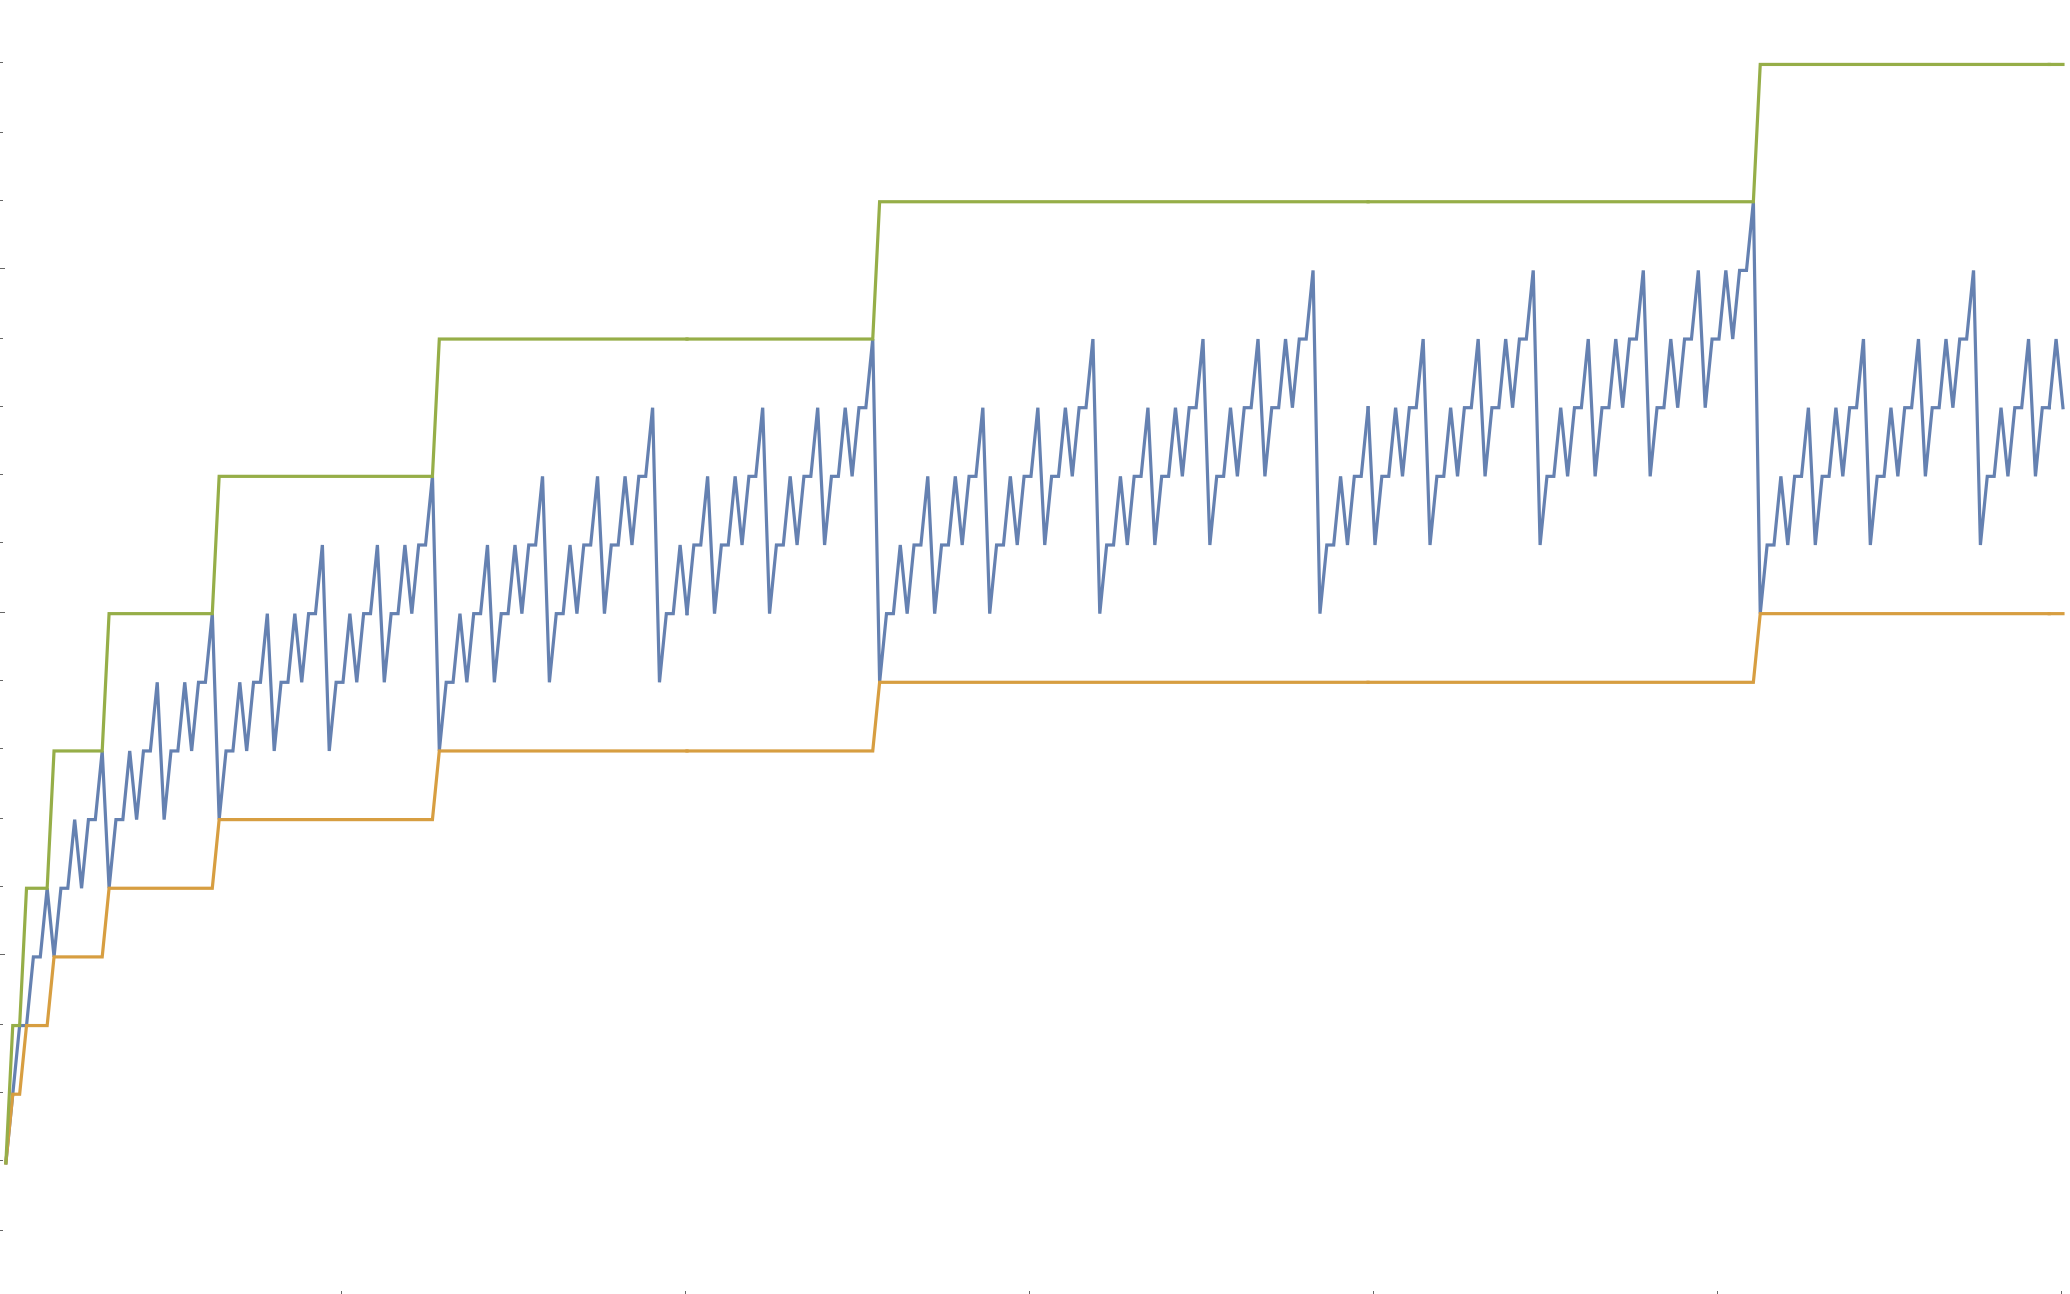
\includegraphics[scale=0.4]{../../Commun/Images/python-cours-complexite-expo-rapide.png}};
\draw[->] (-7.65,-4.3) -- (7.65,-4.3) node[below] {$n$};
\draw[->] (-7.35,-4.6) -- (-7.35,5) node[left] {$C$};
\draw[-] (5.12,-4.2) -- (5.12,-4.4) node[below] {256};
\draw[-] (-7.25,3.15) -- (-7.45,3.15) node[left] {16};
\end{tikzpicture}
\end{center}
Le fait qu'un programme aussi simple ait une complexité au comportement aussi erratique
nous permet de réaliser qu'il est illusoire d'obtenir des formes closes de $C(n)$
pour la plupart des programmes que nous rencontrerons. C'est pourquoi, on se contentera
d'une estimation asymptotique. Malheureusement, l'obtention rigoureuse de ces estimations
est extrêment technique; on se permettra donc de sacrifier une trop grande rigueur
mathématique. Les deux techniques suivantes nous seront très utiles.
\begin{itemize}
\item \emph{Technique de la sommation télescopique}~: Elle consiste à \og résoudre \fg la
  relation de récurrence en se permettant quelques approximations. Dans notre cas,
  on confondra $\ent{n/2}$ et $n/2$ et on écrira $C(n)=C(n/2)+\Theta(1)$, puis
\begin{eqnarray*}
C(n)-C(n/2)&=&\Theta(1)\\
C(n/2)-C(n/4)&=&\Theta(1)\\
\vdots\quad\ \ \qquad&=&\ \ \vdots\\
C(n/2^{k-1})-C(n/2^{k})&=&\Theta(1)
\end{eqnarray*}
  où $k$ est tel que $n/2^{k}\approx 1$, c'est-à-dire $k\approx \log_2 n$. En sommant
  ces égalités, on obtient $C(n)-C(1)=\Theta(1)\log_2 n$, donc $C(n)=\Theta(\log n)$.
\item \emph{Technique de l'arbre d'appels}~: Cette technique commence par faire une
  esquisse de l'arbre d'appels de notre fonction récursive~:
  \begin{center}
  \vspace{2ex}
    \begin{tikzpicture}[level distance = 2.35cm, grow = right]
      \node [ellipse, draw] {$n$}
      child {node [ellipse, draw] {$n/2$}
        child {node [ellipse, draw] {$n/4$}
          child {node [ellipse, draw] {$n/8$}
            child {node [ellipse, draw] {$\cdots$}
                child {node [rectangle, draw] {$n/2^k\approx 1$}}
              }
          }
        }
      }
      ;
    \end{tikzpicture}
  \vspace{2ex}
  \end{center}
  Puisque $n/2^k\approx 1$, on en déduit que $k\approx \log_2 n$. La
  profondeur de notre arbre d'appels est donc de l'ordre de $\log_2 n$. Pour chaque appel,
  on calcule ensuite sa contribution propre à la complexité totale. Autrement dit, on
  estime les opérations élémentaires effectuées par cet appel en ignorant celles
  effectuées par ses enfants. Dans notre cas, chaque appel a une complexité propre
  en $\Theta(1)$. On somme ensuite ces données sur l'ensemble des noeuds de
  l'arbre. Dans notre cas, on obtient une complexité totale en $C(n)=\Theta(1)\log_2 n=
  \Theta(\log n)$.
\end{itemize}
Ces deux techniques sont sur le fond assez semblables, mais la technique de l'arbre
d'appels montrera rapidement sa supériorité lorsque les arbres seront plus
complexes, comme nous allons le voir dans l'exemple suivant.\\

% \begin{exempleUnique}
% \exemple
%   On considère le problème suivant : étant donnée une liste
%   $(u_0,\dots,u_{n - 1})$, renvoyer la liste
%   $(u_0 + n - 1, u_1 + n - 2, \dots, u_{n - 1})$.
%   \begin{itemize}
%     \item \emph{Première version}
% \begin{camlcode}
% let rec f u =
%   match u with
%   | [] -> []
%   | x :: xs -> (x + List.length xs) :: f xs
% \end{camlcode}
%     Si $|u| = n$, alors un appel \verb!f u! donne :
%     \begin{itemize}
%       \item un appel à \verb!f! sur une liste de longueur $n - 1$ ;
%       \item un appel à \verb!List.length! sur une liste de longueur $n - 1$ ;
%       \item des opérations en temps constant.
%     \end{itemize}
%     On en déduit que $T(n) \leq T(n - 1) + An$, avec $A$ une constante.
%     Il vient alors $T(n) = {\rm O}(n^2)$ (en faisant apparaitre une somme télescopique,
%     par exemple), et ce ${\rm O}$ est en fait un $\Theta$.
%     \item \emph{Deuxième version}
% \begin{camlcode}
% let g u =
%   let rec aux u k =
%     match u with
%     | [] -> []
%     | x :: xs -> (x + k) :: aux xs (k - 1) in
%   aux u (List.length u - 1)
% \end{camlcode}
%     Ici, on a :
%     \begin{itemize}
%       \item pour \verb!aux!, en notant $n = |u|$, $T(n) = T(n - 1) + A$
%       et donc $T(n) = \Theta(n)$ ;
%       \item pour \verb!g!, un appel à \verb!List.length! en $\Theta(n)$ et
%       un appel à \verb!aux! en $\Theta(n)$, donc au total $\Theta(n)$.
%     \end{itemize}
%     En réalité, on se contenterait de dire que \verb!g! effectue deux
%     parcours \og~simples~\fg de la liste (un pour \verb!aux! et un pour
%     \verb!List.length!), et est donc en temps linéaire.
%   \end{itemize}
% \end{exempleUnique}

% \subsection{Calculs de complexité amortie}

% Considérons le problème simple de l'incrément d'un compteur binaire, où le coût d'un incrément est
% le nombre de bits à modifier pour passer de l'entier $k$ à son successeur.
% L'incrément est couteux lorsqu'on
% passe de $k\defeq 2^i - 1$  à $2^i$ puisqu'il faut changer $i+1$ bits, mais cette opération coûteuse n'intervient que
% rarement. De plus, elle intervient de plus en plus rarement lorsque $i$ augmente. De plus, les autres opérations
% sont peu coûteuses. Par exemple, passer d'un nombre pair à son successeur implique un coût unitaire. Le coût de l'incrémentation est ${\rm O}\p{\log k}$.
% Cependant, nous allons montrer que le coût amorti de \verb!incr! est constant.
% Plusieurs méthodes permettent de mettre en place le calcul d'un coût amorti.\\

% \begin{itemize}
% \item \emph{L'analyse cumulée}~: Avec cette méthode, on calcule le temps total $C(n)$ pour effectuer $n$ opérations
%   et on conclut que le coût amorti est $C(n)/n$. Si on reprend l'exemple de l'incrément binaire, en effectuant $n$ incréments
%   successifs en commençant à l'entier $k=0$, et en notant $\underline{b_{p-1} \ldots b_0}_2$ la représentation binaire de
%   notre nombre
%   \begin{itemize}
%   \item $b_0$ est modifié à chaque incrément.
%   \item $b_1$ est modifié $\ent{n/2}$ fois.
%   \item Plus généralement, $b_i$ est modifié $\ent{n/2^i}$ fois.
%   \end{itemize}
%   Le coût total est donc de
%   \[C(n)=\sum_{i=0}^{+\infty} \ent{\frac{n}{2^i}}\leq n \sum_{i=0}^{+\infty} \frac{1}{2^i} = 2n\]
%   ce qui donne un coût amorti constant.
% \item \emph{La méthode comptable}~: Cette méthode consiste à affecter à chaque opération un coût amorti. Si le coût
%   amorti d'une opération est plus grand que le coût réel, alors la différence, appelé \emph{crédit} permet de payer pour les
%   opérations futures dont le coût réel est supérieur au coût amorti. Lorsque l'on choisit les coûts amortis, il est nécessaire
%   de s'assurer que toute suite de $n$ opérations donne toujours un coût amorti supérieur au coût réel. Dans le cas de
%   notre incrémentation binaire, on peut la décomposer en deux opérations élémentaires.
%   \begin{itemize}
%   \item Le bit $b_i$ passe de 0 à 1~: le coût réel est de 1 et on affecte un coût amorti de 2. Le crédit vaut alors 1.
%   \item Le bit $b_i$ passe de 1 à 0~: le coût réel est de 1, on affecte un coût amorti de 0 et on utilise le crédit de l'opération
%     précédente.
%   \end{itemize}
%   Le crédit total est toujours positif car il correspond au nombre total de bits égaux à 1. De plus, puisque chaque incrémentation
%   change au plus un bit de 0 à 1, le coût amorti est constant.
% \item \emph{La méthode du potentiel}~: C'est la méthode la plus utilisée en pratique. On débute avec une structure de donnée
%   $d_0$ sur laquelle on va effectuer $n$ opérations de coût réel $c_i$ pour $i\in\intere{1}{n}$. On note $d_i$ la structure
%   obtenue après la $i$-ième opération. Une fonction potentiel $\Phi$ affecte à chaque structure un réel positif $\Phi(d_i)$
%   assimilable à l'énergie potentielle de la structure de donnée. On définit alors le coût amorti $\hat{c_i}$ pour l'opération $i$
%   par
%   \[\hat{c_i} = c_i + \Phi(d_i) - \Phi(d_{i - 1}).\]
%   Sur les $n$ opérations, le coût amorti total est donc égal à
%   \[\sum_{i=1}^n \hat{c_i} = \sum_{i=1}^n c_i + \Phi\p{d_n} - \Phi\p{d_0}\]
%   Nous choisirons des fonctions potentielles pour lesquelles $\Phi(d_n)\geq\Phi(d_0)$. On a donc
%   \[\sum_{i=1}^n c_i \leq \sum_{i=1}^n \hat{c_i}.\]
%   Pour que cette méthode soit efficace, il faut trouver une bonne fonction potentiel, en ce sens qu'elle doit accumuler
%   de l'énergie pour les opérations de faible coût réel pour pouvoir en libérer sur les structures sur lesquelles le coût des
%   opérations est élevé. Dans notre exemple précédent, on note $\Phi(k)$ le nombre de 1 dans la représentation binaire de $k$.
%   On note $u_i$ le nombre des bits à 1  après la $i$-ième incrémentation et $z_i$ le nombres de bits mis à 0 à la
%   $i$-ième incrémentation. On a alors $u_i=u_{i-1}-z_i+1$ et donc
%   \[\hat{c_i}=c_i + \Phi(d_i) - \Phi(d_{i - 1})=2.\]
%   Le coût amorti d'une incrémentation est donc en ${\rm O}(1)$.
% \end{itemize}

Nous allons revenir sur l'algorithme de tri fusion dont nous rappelons le code ici. On
commence par remarquer que la fonction \verb!fusion(t1, t2)! a une complexité en
$\Theta(|t_1|+|t_2|)$. En effet, chaque passage dans la boucle \verb!while! ajoute un
élément parmi les listes $t_1$ et $t_2$ à notre liste $t$. Les appels à \verb!extend!
ajoutent les éléments restants une fois qu'une des deux listes est épuisée.
\begin{pythoncodeline}
def fusion(t1, t2):
    """fusion(t1: list[int], t2: list[int]) -> list[int]"""
    t = []
    i1 = 0
    i2 = 0
    while i1 < len(t1) and i2 < len(t2):
        if t1[i1] < t2[i2]:
            t.append(t1[i1])
            i1 = i1 + 1
        else:
            t.append(t2[i2])
            i2 = i2 + 1
    t.extend(t1[i1:])
    t.extend(t2[i2:])
    return t
\end{pythoncodeline}

\begin{pythoncodeline}
def tri_fusion(t):
    """tri_fusion(t: list[int]) -> list[int]"""
    n = len(t)
    if n <= 1:
        return t[:]
    n1 = n // 2
    t1 = tri_fusion(t[0:n1])
    t2 = tri_fusion(t[n1:n])
    t = fusion(t1, t2)
    return t
\end{pythoncodeline}
Si on note $C(n)$ la complexité de la fonction \verb!tri_fusion!,
on a donc
\[C(n)=C(\ent{n/2}) + C(\ents{n/2})+\Theta(n).\]
Pour obtenir une estimation asymptotique de $C(n)$, nous allons utiliser la technique
de l'arbre d'appels. La racine représente l'appel initial à \verb!tri_fusion! 
avec une liste de taille $n$, qui
appelle récursivement notre fonction avec des listes de taille $n/2$, qui elles-mêmes appellent
récursivement notre fonction avec des listes de taille $n/4$, etc. 
\begin{center}
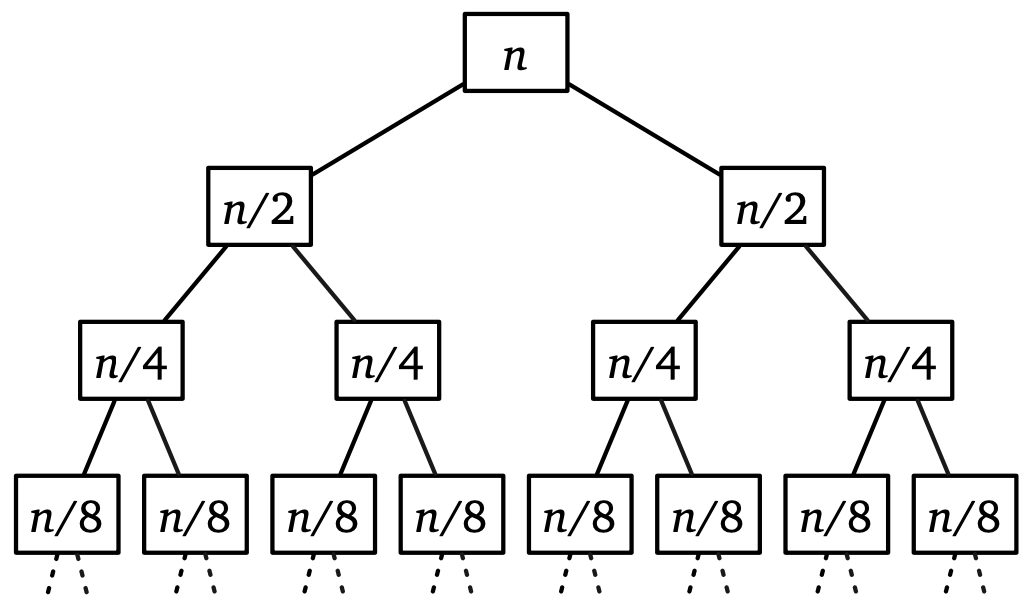
\includegraphics[width=0.35\textwidth]{../../Commun/Images/python-cours-merge}
\end{center}
On tombe sur un cas de base lorsque la taille des listes est inférieure ou égale à 1.
La hauteur $h$ de cet arbre vérifie donc $n/2^h \approx 1$, ce qui nous donne
$h\approx \log_2 n$.
Pour estimer la complexité de l'appel initial, il suffit désormais de
prendre en compte le cout propre de chaque appel, c'est-à-dire le cout de la fusion. Pour
simplifier le calcul, on va sommer ligne par ligne.
\begin{itemize}
\item Sur la première ligne, on compte une fusion pour une liste de taille $n$; ce cout est de $\Theta(n)$.
\item Sur la seconde ligne,
on compte 2 fusions pour des listes de taille $n/2$; ce cout est de
$2\Theta(n/2)=\Theta(n)$.
\item Sur la troisième ligne, on compte 4 fusions pour des listes
de taille $n/4$; ce cout est de $4\Theta(n/4)=\Theta(n)$.
\end{itemize}
On constate que sur chaque
ligne, le cout est de $\Theta(n)$. Comme l'arbre est de hauteur $\log_2 n$, on en déduit
que la complexité du tri fusion est de $C(n)=\Theta(n)\log_2 n=\Theta(n\log n)$.

\section{Calcul de complexité spatiale}

\subsection{Algorithme itératif}

La complexité en espace mesure la quantité de mémoire de travail utilisée
par l'algorithme. On ne compte pas la taille des données.\\

La fonction suivante calcule le $n$-ième nombre de Fibonacci pour $n\geq 1$~:
\begin{pythoncodeline}
def fibo(n):
    """fibo(n: int) -> int"""
    t = [None] * (n + 1)
    t[0] = 0
    t[1] = 1
    for i in range(2, n + 1):
        t[i] = t[i - 1] + t[i - 2]
    return t[n]
\end{pythoncodeline}
          Elle a une complexité en espace en $\Theta(n)$ puisqu'elle
          alloue un tableau de taille $n + 1$ pour réaliser ses
          calculs. Sa complexité en temps est également linéaire.\\

La fonction suivante effectue le même calcul :

\begin{pythoncodeline}
def fibo(n):
    """fibo(n: int) -> int"""
    u = 0
    v = 1
    for _ in range(n):
        u, v = v, u + v
    return u
\end{pythoncodeline}
          Elle a également une complexité temporelle linéaire,
          mais sa complexité spatiale est constante, puisqu'elle
          utilise uniquement deux variables entières.\\



De nombreux algorithmes \og échangent de l'espace contre du temps \fg : pour obtenir une meilleure
complexité temporelle, on accepte une moins bonne complexité spatiale. C'est par exemple le cas
de tous les algorithmes de programmation dynamique, que nous étudierons ultérieurement.
C'est souvent efficace en pratique, mais il
y a un certain nombre de seuils qu'il est couteux de dépasser~: les données ne rentrent plus dans
le cache, les données ne rentrent plus en mémoire vive, les données ne rentrent plus dans le
stockage de masse local, etc.\\

\noindent
\emph{Taille des données et capacité des mémoires}~:
Il faut avoir en tête quelques ordres de grandeur~:
\begin{itemize}
  \item Un entier ou un flottant prennent en général 8 octets en mémoire.
  \item Un ordinateur typique a quelques gigaoctets de mémoire vive.
  \item Ce même ordinateur peut disposer de quelques téraoctets de mémoire
  de stockage, mais si l'on doit utiliser cette mémoire pour les calculs,
  les performances peuvent facilement être divisées par mille, voire un million.
\end{itemize}



\subsection{Algorithme récursif}

% Dans cette partie, on utilisera autant \textsc{OCaml} que C pour illustrer les
% concepts : certaines questions ne se posent qu'en C, mais la plupart
% sont les mêmes dans tous les langages.

\subsubsection{Pile d'appels}

Considérons les deux fonctions suivantes

\begin{pythoncodeline}
def g(n):
    """g(n: int) -> int"""
    return n * n

def f(n):
    """f(n: int) -> int"""
    s = 0
    for k in range(1, n + 1):
        s = s + g(k)    # .L104
    return s
\end{pythoncodeline}

% \begin{camlcode}[numbers = left]
% let g n =
%   n * n

% let f n =
%   let s = ref 0 in
%   let k = ref 1 in
%   while !k <= n do
%     s := !s + g !k;   (* .L104 *)
%     incr k
%   done;
%   !s
% \end{camlcode}
\noindent
Voici l'état de la pile d'appels lors du premier passage ligne 9 dans le
calcul de $f(10)$.
  % \begin{figure}[H]
  %   \centering
    \begin{center}
    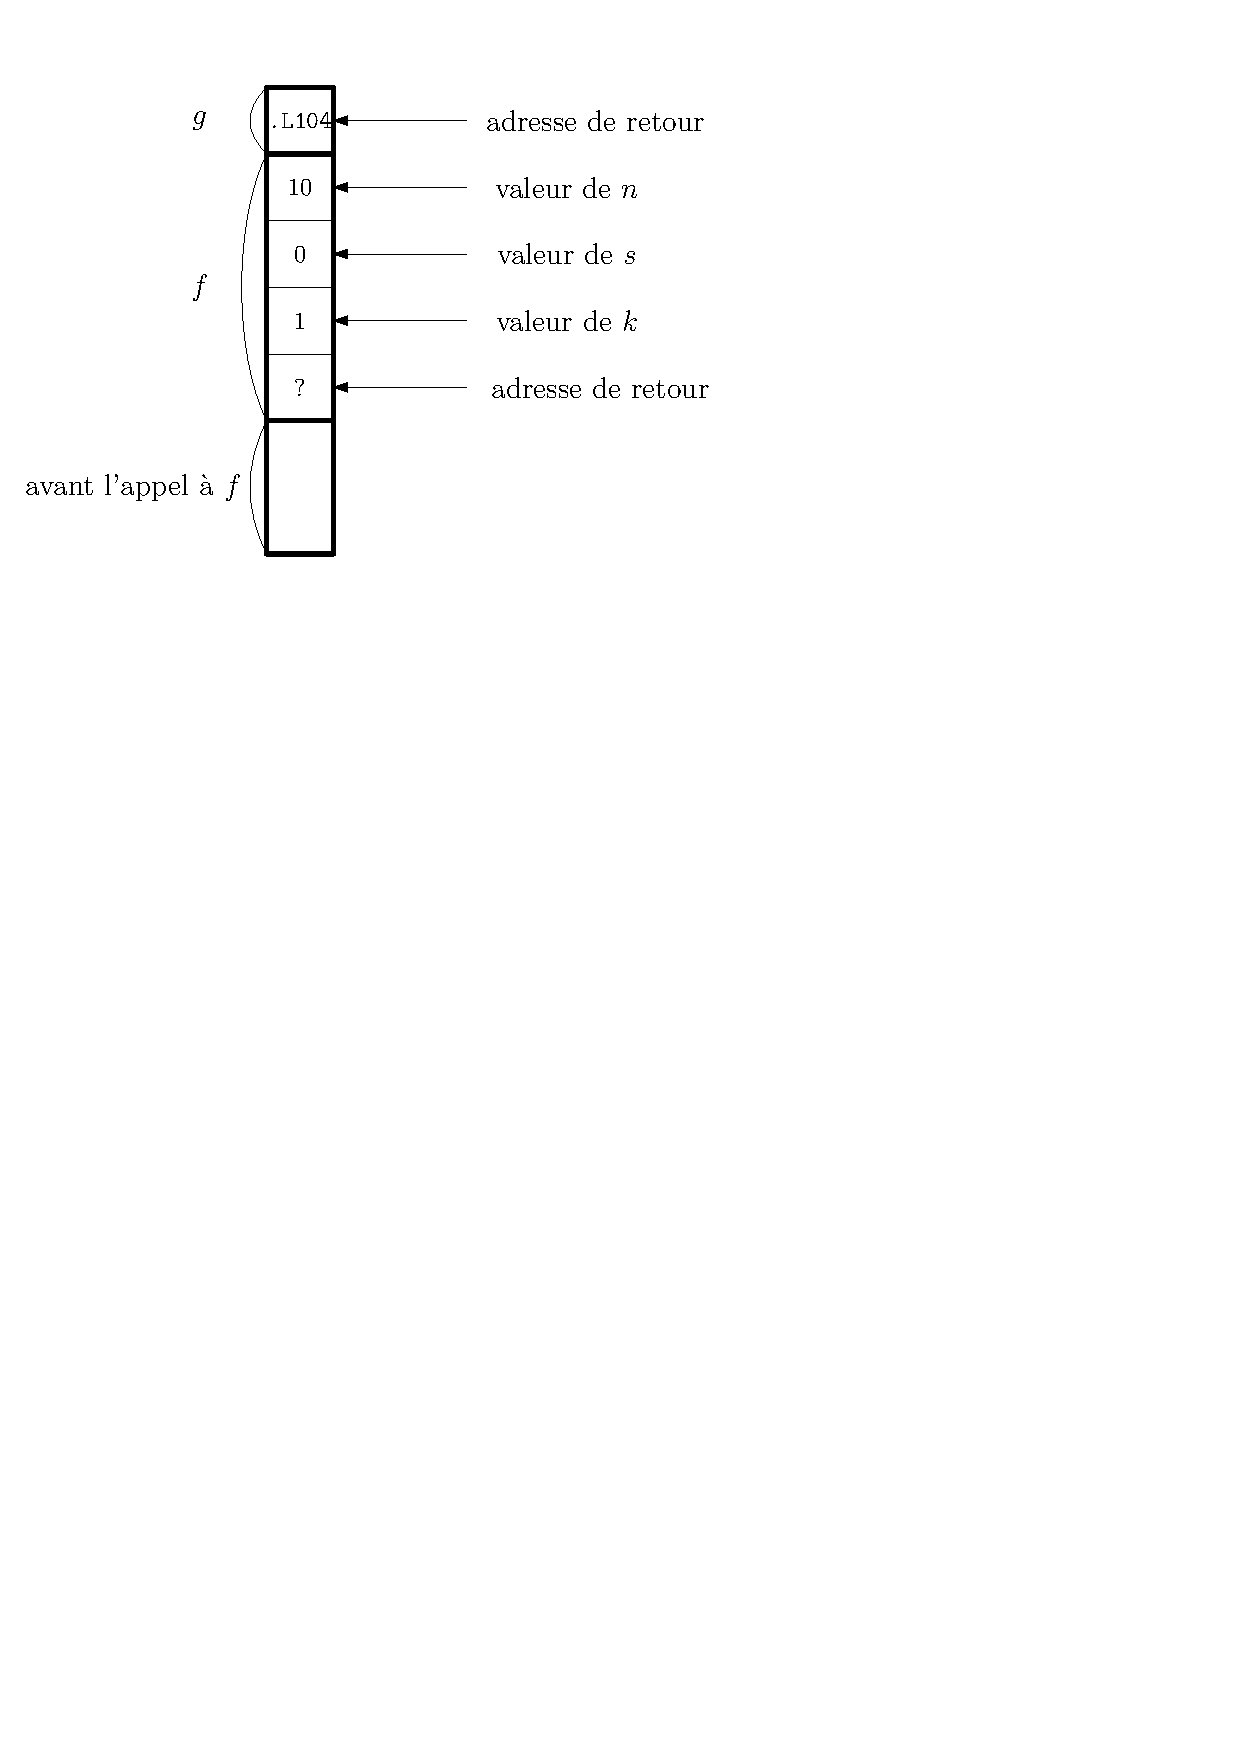
\includegraphics[page = 1, width = 7.5cm]{../../Commun/Images/info-cours-complexite_pile}
    \end{center}
  %   \label{fig:pile-appels}
  % \end{figure}

Que se passe-t-il \og en vrai \fg quand on calcule $f(2)$ ? $f$ crée des
variables locales, leur donne une valeur, puis appelle $g$ avec l'argument $1$.
Pour cela, elle cède le contrôle d'exécution à $g$ et l'exécution \og saute \fg au
début du code de $g$. Quand $g$ aura fini son calcul, il faudra qu'elle rende
la main à $f$ : mais l'exécution de $f$ doit reprendre là où elle s'est arrêtée,
et dans l'environnement qui était valable à ce moment~: \verb!s! doit valoir $0$,
\verb!k! doit valoir $1$, etc. Il faut donc que $f$ sauvegarde un certain nombre
d'informations avant d'appeler $g$.\\

Cette sauvegarde d'informations se fait sur la \emph{pile
  d'appels}.
Vu de loin, un élément (on parle de \emph{stackframe} ou \emph{bloc d'activation})
de la pile contient
toutes les informations relatives à un appel donné d'une fonction donnée :
\begin{itemize}
  \item Les arguments de la fonction
  \item Les variables locales de la fonction.
  \item Le point auquel l'exécution du programme devra reprendre quand
        l'appel sera terminé.
\end{itemize}\smallskip

Quand une fonction est appelée, elle crée une
\emph{stackframe}
   au sommet de
la pile, qu'elle supprimera juste avant de renvoyer son résultat et de passer
le contrôle au point qui était sauvegardé. À tout moment de l'exécution du
programme, la hauteur de la pile (en nombre de \emph{frames}) est donc égale au
nombre de fonctions actives, c'est-à-dire ayant été appelées et n'ayant pas
encore retourné leur résultat.\\

Une remarque sur la terminologie : le nom de \og pile \fg n'est bien sûr pas anodin,
il y a bien une très forte analogie avec la structure de données que nous avons
vue. On empile au moment des appels, on dépile au moment
des retours.
% Seul le bloc d'activation situé au sommet de la pile est actif~: la fonction n'a pas accès aux variables locales de la fonction appelante !
% En revanche, on peut accéder sans problème
% à n'importe quelle variable située dans ce bloc au sommet.

% \subsubsection{Un coup d'œil sous le capot}

% On peut demander à \textsc{OCaml} de nous donner l'assembleur généré à la compilation
% d'un fichier. Dans les multiples transformations que subit un programme
% avant de pouvoir être exécuté, celle qui
% fournit l'assembleur est essentiellement l'avant-dernière : le programme est
% encore lisible par un humain (avec un peu de bonne volonté), mais sa traduction
% en langage machine est \og triviale \fg.
% % \begin{figure}[H]
% %   \centering
%   \begin{center}
%   \includegraphics[page = 2, width = 14cm]{../../Commun/Images/info-cours-complexite_pile}
%   \end{center}
% %   \caption{Étapes de la compilation d'un programme \textsc{OCaml}.}
% % \end{figure}

% % \begin{figure}[H]
%   \begin{center}
% \begin{asmcode}
% 0000000000417050 <camlAsm1__g_8>:
%   417050:       48 89 c3                mov    rbx,rax
%   417053:       48 d1 fb                sar    rbx,1
%   417056:       48 ff c8                dec    rax
%   417059:       48 0f af c3             imul   rax,rbx
%   41705d:       48 ff c0                inc    rax
%   417060:       c3                      ret
% \end{asmcode}
%   % \caption{Récupération de l'assembleur (à droite) à partir du code machine
%   %   (au milieu).}
% \end{center}

% \noindent Voyons donc ce que produit \textsc{OCaml} sur cet
% exemple. Notons que l'assembleur a été nettoyé et simplifié.
% \begin{nasmcode}
% Fonction_g:
% .L100:
%     movq    %rax, %rbx     ; On élève l'argument au carré
%     ...                    ; (c'est un peu compliqué pour des
%     imulq   %rbx, %rax     ; raisons techniques).
%     ret                    ; On renvoie et l'on saute au point de retour
%                            ; sauvegardé.
% Fonction_f:
%     subq    $24, %rsp      ; On réserve de la place sur la pile pour 3 entiers.
% .L103:
%     ...                    ; Je saute l'initialisation.
% .L102:
%     movq    (%rsp), %rdi   ; On charge n dans %rdi.
%     cmpq    %rdi, %rax     ; On compare n et k.
%     jg      .L101          ; Si k > n, on sort de la boucle.
%     call    Fonction_g     ; Sinon, on appelle g (en sauvegardant le point de
%                            ; retour)
% .L104:
%     movq    8(%rsp), %rbx  ; On restaure s.
%     addq    %rax, %rbx     ; On ajoute à s le résultat de g.
%     ...
%     movq    %rbx, 8(%rsp)  ; On sauvegarde s (pour le prochain appel).
%     movq    16(%rsp), %rax ; On restaure k.
%     addq    $2, %rax       ; On incrémente k.
%     movq    %rax, 16(%rsp) ; On sauvegarde k (pour le prochain appel).
%     jmp     .L102          ; On retourne au début de la boucle.
% .L101:
%     movq    %rbx, %rax     ; On prépare le résultat.
%     addq    $24, %rsp      ; On libère la pile.
%     ret                    ; On renvoie et l'on saute au point de retour
%                            ; sauvegardé.
% \end{nasmcode}


\subsubsection{Pile et fonction récursive}

Pour l'instant, on a considéré le cas d'une fonction $f$ qui
appelle une fonction $g$. Mais rien n'empêche bien sûr $f$
de s'appeler elle-même : ce sera le cas si $f$
est récursive. Dans ce cas, il y aura
\emph{un bloc d'activation par appel actif de $f$}.
C'est logique, puisque chacun de ses appels possède ses propres variables
locales, et son propre compteur de programme étant donné que chacun des appels en est à un
point différent de son exécution.\\

Pour visualiser ce type de situation, il est plus intéressant de réfléchir en
termes d'\emph{arbres d'appels}. Considérons une fonction calculant les termes
de la suite de Fibonacci de manière récursive et naïve. Ici, \og naïve \fg
  est à comprendre au sens de \emph{scandaleusement
    mauvais et contraire aux bonnes mœurs}.
\begin{pythoncodeline}
def fib(n):
    """fib(n: int) -> int"""
    if n <= 1:
        return n
    else:
        return fib(n - 1) + fib(n - 2)
\end{pythoncodeline}
% \begin{camlcode}
% let rec fib n =
%   if n <= 1 then n
%   else fib (n - 2) + fib (n - 1)
% \end{camlcode}
Un appel à \verb!fib(5)! produit un appel à \verb!fib(4)! et un à \verb!fib(3)!,
qui produisent eux-mêmes d'autres appels, etc. La situation est très bien
résumée par l'arbre d'appels suivant pour \verb!fib(5)!.
% \begin{figure}[H]
%   \centering
\begin{center}
  \begin{tikzpicture}[level/.style = {level distance = .5cm,
      sibling distance = 8cm/#1},
    every node/.style = draw]
\node [ellipse, draw] {\texttt{fib 5}}
child {node [ellipse] {\texttt{fib 4}}
child {node [ellipse] {\texttt{fib 3}}
child {node [ellipse] {\texttt{fib 2}}
child {node [rectangle] {\texttt{fib 1}}}
child {node [rectangle] {\texttt{fib 0}}}
}
child {node [rectangle] {\texttt{fib 1}}}
}
child {node [ellipse] {\texttt{fib 2}}
child {node [rectangle] {\texttt{fib 1}}}
child {node [rectangle] {\texttt{fib 0}}}
}
}
child {node [ellipse] {\texttt{fib 3}}
child {node [ellipse] {\texttt{fib 2}}
child {node [rectangle] {\texttt{fib 1}}}
child {node [rectangle] {\texttt{fib 0}}}
}
child {node [rectangle] {\texttt{fib 1}}}
}
;
  \end{tikzpicture}
\end{center}


\noindent
Voici l'évolution de la pile d'appels lors du calcul de \verb!fib(5)!.

% \begin{multicols}{2}
% \begin{figure}[H]
%   \centering
\begin{center}
  \begin{multicols}{2}
\begin{verbatim}
    fib(5)
    fib(5) | fib(4)
    fib(5) | fib(4) | fib(3)
    fib(5) | fib(4) | fib(3) | fib(2)
    fib(5) | fib(4) | fib(3) | fib(2) | fib(1)
    fib(5) | fib(4) | fib(3) | fib(2)
    fib(5) | fib(4) | fib(3) | fib(2) | fib(0)
    fib(5) | fib(4) | fib(3) | fib(2)
    fib(5) | fib(4) | fib(3)
    fib(5) | fib(4) | fib(3) | fib(1)
    fib(5) | fib(4) | fib(3)
    fib(5) | fib(4)
    fib(5) | fib(4) | fib(2)
    fib(5) | fib(4) | fib(2) | fib(1)
--> fib(5) | fib(4) | fib(2)
    fib(5) | fib(4) | fib(2) | fib(0)
    fib(5) | fib(4) | fib(2)
    fib(5) | fib(4)
    fib(5)
    fib(5) | fib(3)
    fib(5) | fib(3) | fib(2)
    fib(5) | fib(3) | fib(2) | fib(1)
    fib(5) | fib(3) | fib(2)
    fib(5) | fib(3) | fib(2) | fib(0)
    fib(5) | fib(3) | fib(2)
    fib(5) | fib(3)
    fib(5) | fib(3) | fib(1)
    fib(5) | fib(3)
    fib(5)
\end{verbatim}
\vspace{3ex}
\begin{tikzpicture}[level/.style = {level distance = 1.5cm,
  sibling distance = 6cm/#1},
every node/.style = draw]
\node [ellipse, fill = colorLazoYellow1Light] {\texttt{fib(5)}} [grow=right]
child {node [ellipse, fill = colorLazoYellow1Light] {\texttt{fib(4)}}
child {node [ellipse, fill = black!10] {\texttt{fib(3)}}
child {node [ellipse, fill = black!10] {\texttt{fib(2)}}
child {node [rectangle, fill = black!10] {\texttt{fib(1)}}}
child {node [rectangle, fill = black!10] {\texttt{fib(0)}}}
}
child {node [rectangle, fill = black!10] {\texttt{fib(1)}}}
}
child {node [ellipse, fill = colorLazoBlue2Light] {\texttt{fib(2)}}
child {node [rectangle, fill = black!10] {\texttt{fib(1)}}}
child {node [rectangle] {\texttt{fib(0)}}}
}
}
child {node [ellipse] {\texttt{fib(3)}}
child {node [ellipse] {\texttt{fib(2)}}
child {node [rectangle] {\texttt{fib(1)}}}
child {node [rectangle] {\texttt{fib(0)}}}
}
child {node [rectangle] {\texttt{fib(1)}}}
}
;
\end{tikzpicture}
\end{multicols}
\end{center}



% \begin{center}

% \end{center}

Il faut avoir de cet arbre une vision dynamique : on en effectue un parcours en
profondeur. Quand on est en train de visiter un n\oe ud, les appels actifs sont
ceux correspondant au n\oe ud actuel ainsi qu'à tous ses ancêtres,
c'est-à-dire
tous les n\oe uds situés sur le chemin qui le relie à la racine.
% C'est ce qui
% est illustré par les figures~\ref{fig:evolution-pile-appels} et
% \ref{fig:arbre-evolution-pile-appels}.
% Notons que l'on peut très facilement obtenir une \og trace \fg des appels à une
% fonction dans la boucle interactive de Python. Une fois que l'on a défini une
% fonction (disons \verb!fibo!) il suffit d'exécuter \verb!#trace fibo!
% (avec le \verb!#! !) pour qu'un appel à \verb!fibo! affiche tous les appels
% engendrés.
% \begin{camlcode}
% # #trace fibo;;
% fibo is now traced.
% # fibo 4;;
% fibo <-- 4 # appel à fibo 4
% fibo <-- 3 # appel à fibo 3
% fibo <-- 2 # appel à fibo 2
% fibo <-- 1 # appel à fibo 1
% fibo --> 1 # fibo 1 -> 1
% fibo <-- 0
% fibo --> 0
% fibo --> 1
% fibo <-- 1
% fibo --> 1
% \end{camlcode}
% \begin{camlcode}
% fibo --> 2 # fibo 3 -> 2
% fibo <-- 2 # appel à fibo 2
% fibo <-- 1 # ...
% fibo --> 1 # ...
% fibo <-- 0 # ...
% fibo --> 0 # ...
% fibo --> 1 # qui finit par renvoyer 1
% fibo --> 3 # l'appel initial renvoie 3
% - : int = 3
% # #untrace fibo;;
% fibo is no longer traced.
% # fibo 4;;
% - : int = 3
% \end{camlcode}
La hauteur maximale de la pile est égale à la hauteur de l'arbre.
Ici, cette hauteur est de l'ordre de $n$ alors que le temps d'exécution est
exponentiel.\\

\begin{exoUnique}
\exo Montrer que la complexité temporelle de la fonction \verb!fib! est en
\[\Theta(\phi^n)\]
où $\phi\defeq(1+\sqrt{5})/2$ est le nombre d'or.
\end{exoUnique}
\vspace{2ex}

Cependant, si l'on s'intéresse à une fonction ayant une structure
d'appels plus simple, les choses peuvent être différentes.
\begin{pythoncodeline}
def somme(n):
    """somme(n: int) -> int"""
    if n == 0:
        return 0
    else:
        return n + somme(n - 1)
\end{pythoncodeline}
Ici, l'arbre d'appels obtenu est en fait linéaire. Voici par exemple l'arbre d'appels
pour \verb!somme(6)!~:
\begin{center}
  \begin{tikzpicture}[level distance = 2.35cm, grow = right]
    \node [ellipse, draw] {\small \texttt{somme 6}}
    child {node [ellipse, draw] {\small \texttt{somme 5}}
      child {node [ellipse, draw] {\small \texttt{somme 4}}
        child {node [ellipse, draw] {\small \texttt{somme 3}}
          child {node [ellipse, draw] {\small \texttt{somme 2}}
            child {node [ellipse, draw] {\small \texttt{somme 1}}
              child {node [rectangle, draw] {\small \texttt{somme 0}}}
            }
          }
        }
      }
    }
    ;
  \end{tikzpicture}
\end{center}
Le problème, qui n'est pas forcément évident quand on regarde le code,
est qu'un appel à \verb!somme(n)! demande un espace mémoire proportionnel
à $n$ : c'est la hauteur maximale de la pile d'appels.
De plus, l'espace disponible sur la pile est bien plus limité que
l'espace mémoire total. Le résultat :
\begin{pythoncode}
In [1]: somme(3000)
(*@\textcolor{purple}{RecursionError: maximum recursion depth exceeded in comparison}@*)
\end{pythoncode}
Notons que le temps de calcul n'est pas le problème : le \emph{stackoverflow}
 se produit presque instantanément.
\begin{proposition}
  La complexité en espace d'une fonction récursive est au moins égale à sa
  profondeur maximale de récursion, c'est-à-dire à la profondeur de son arbre
  d'appels.
\end{proposition}
\begin{remarques}
  \remarque Elle peut bien sûr être supérieure à cette profondeur, typiquement si la
  fonction crée des listes auxiliaires.
  \remarque Par défaut, l'espace disponible sur la pile est assez faible, de l'ordre de quelques mégaoctets. On peut donc faire un
  \emph{stackoverflow} bien avant d'épuiser la mémoire disponible.
\end{remarques}

Ici, cette complexité linéaire en espace est problématique : une fonction itérative
aura clairement une utilisation mémoire constante, sauf si l'on s'amuse à stocker tous les
résultats intermédiaires.

\begin{pythoncodeline}
def somme(n):
    """somme(n: int) -> int"""
    s = 0
    for k in range(1, n + 1):
        s += k
    return s
\end{pythoncodeline}

\noindent Et le problème disparait :
\begin{pythoncode}
In [2]: somme(3000)
Out[2]: 4501500 
\end{pythoncode}

% \subsubsection{Récursion terminale}


% En Python, on s'arrêterait là : si une fonction a une
% structure d'appel aussi simple, il est facile de la \og dé-récursifier \fg, et on
% évite les problèmes de \emph{stack overflow}. Cependant, la programmation
% fonctionnelle, et donc le \textsc{OCaml}, se prête plus facilement à un style récursif
% qu'itératif. Par conséquent, le compilateur \textsc{OCaml} procède à une optimisation
% appelée \emph{élimination de la récursion terminale}.

% \begin{remarqueUnique}
%   \remarque
%   \verb!gcc! et \verb!clang! procèdent également tous les deux à cette
%   optimisation. Cependant, elle n'est pas garantie par le standard C,
%   et il n'est pas \emph{a priori} impossible que le compilateur la
%   \og manque \fg dans certains cas, par exemple parce qu'il a d'abord
%   procédé à une autre optimisation. En \textsc{OCaml}, l'élimination est garantie.
% \end{remarqueUnique}
% \vspace{2ex}
% Si l'on regarde le code de la fonction \verb!somme!, on voit qu'il est
% indispensable de sauvegarder le contexte avant de procéder à l'appel récursif.
% En effet, le résultat de cet appel devra être ajouté à $n$, dont il faut 
% se rappeler la valeur, avant d'être renvoyé par la fonction appelante. En
% revanche, considérons la fonction suivante :
% \begin{camlcode}
% let somme_terminale n =
%   let rec somme_aux n acc =
%     if n > 0 then somme_aux (n - 1) (acc + n)
%     else acc in
%   somme_aux n 0
% \end{camlcode}
% La fonction \verb!somme_terminale! n'est pas récursive et n'est appelée qu'une
% fois, on peut donc l'ignorer. La fonction \verb!somme_aux!, qui effectue
% véritablement le calcul, n'a qu'un seul appel récursif, \emph{dont elle
%   renvoie immédiatement le résultat}. Comme elle n'aura aucun travail à
% effectuer une fois l'appel récursif terminé, il est totalement inutile de
% sauvegarder son contexte. Le compilateur le remarque, et elle s'exécute
% maintenant en espace constant.
% \begin{camlcode}
% # somme_terminale 1_000_000;;
% - : int = 500000500000
% \end{camlcode}

% \begin{definition}
%   Une fonction est dite \emph{récursive terminale} (ou \emph{tail recursive})
%   si les seuls appels récursifs qu'elle contient sont placés en position
%   finale, c'est-à-dire si elle renvoie immédiatement le résultat sans faire
%   d'opération dessus.\\

%   En \textsc{OCaml}, une telle fonction sera automatiquement compilée en une version non
%   récursive et ne pourra donc jamais donner lieu à un dépassement de pile.
% \end{definition}

% \begin{remarques}
%   \remarque La plupart des langages fonctionnels font la m\^{e}me optimisation que
%   \textsc{OCaml}, car la récursion y est souvent utilisée pour faire ce genre de calculs
%   (dans certains de ces langages, c'est même la seule possibilité). En revanche, dans
%   un langage comme Python, le fait qu'une fonction récursive soit terminale ou
%   pas ne change rien : si l'on veut écrire une fonction \verb!max! qui
%   fonctionne sur des listes \og longues \fg, on est donc obligé de le faire avec
%   une boucle.
%   \remarque Une fonction récursive terminale n'est en quelque sorte \og pas vraiment
%   récursive \fg : il est en effet très facile de la transformer en une fonction
%   non récursive utilisant juste un accumulateur et une boucle \verb!while!.
%   C'est ce que le compilateur fait automatiquement.
%   \remarque Toute fonction récursive peut être rendue terminale (et donc
%   dé-récursifiée), mais le plus souvent cela revient simplement à programmer
%   \og à la main \fg la pile d'appels, ce qui a pour principal intérêt de rendre le
%   code complètement incompréhensible.
% \end{remarques}


% On reprend les deux fonctions récursives calculant la somme des $n$ premiers entiers.

% \begin{camlcode}
% let rec somme n =
%   if n > 0 then n + somme (n - 1)
%   else 0
% \end{camlcode}

% \begin{camlcode}
% let somme_terminale n =
%   let rec somme_aux n acc =
%     if n > 0 then somme_aux (n - 1) (acc + n)
%     else acc in
%   somme_aux n 0
% \end{camlcode}

% \noindent On considère aussi une version itérative, et l'assembleur généré par
% \textsc{OCaml} pour cette version.
% \begin{camlcode}
% let somme_iter n =
%   let s = ref 0 in
%   let k = ref n in
%   while !k > 0 do
%     s := !s + !k;
%     decr k
%   done;
%   !s
% \end{camlcode}

% \begin{asmcode}
% Fonction somme_iter:
% .L108:
%         movq    $1, %rbx             ; s <- 0
% .L107:
%         cmpq    $1, %rax             ; si k <= 0
%         jle     .L106                ; aller en L106
%         leaq    -1(%rbx,%rax), %rbx  ; sinon, s <- s + k
%         addq    $-2, %rax            ; k <- k - 1
%         jmp     .L107                ; aller en L107
% .L106:
%         movq    %rbx, %rax           ; on se prépare à renvoyer s
%         ret                          ; on renvoie
% \end{asmcode}


% Les deux fonctions récursives sont compilées très différemment,
% mais le point crucial est que la version récursive terminale
% est compilée exactement de la même manière que la version itérative.

% \begin{asmcode}
% Fonction somme:
%         subq    $8, %rsp             ; on réserve une place sur la pile
% .L102:
%         cmpq    $1, %rax             ; si n <= 0
%         jle     .L101                ; alors on va en L101
%         movq    %rax, (%rsp)         ; sinon, on sauvegarde n
%         addq    $-2, %rax            ;
%         call    somme                ; puis on appelle somme (n - 1)
% .L100:
%         movq    (%rsp), %rbx         ; on restaure n
%         leaq    -1(%rbx,%rax), %rax  ; on l'ajoute au résultat de l'appel
%         addq    $8, %rsp             ; on libère la pile
%         ret                          ; et on renvoie
% .L101:
%         movq    $1, %rax             ; on se prépare à renvoyer 0
%         addq    $8, %rsp             ; on libère la pile
%         ret                          ; on renvoie
% Fonction somme_aux:
% .L113:
%         cmpq    $1, %rax             ; si n <= 0
%         jle     .L112                ; on va en L112
%         leaq    -1(%rbx,%rax), %rbx  ; sinon, acc <- acc + n
%         addq    $-2, %rax            ; n <- n - 1
%         jmp     .L113                ; on va en L113
% .L112:
%         movq    %rbx, %rax           ; on se prépare à renvoyer acc
%         ret                          ; on renvoie
% Fonction somme_term:
% .L110:
%         movq    $1, %rbx             ; acc <- 0
%         jmp     L113                 ; on appelle somme_aux (appel terminal)
% \end{asmcode}

% Les deux manières de calculer la somme sont compilées très différemment.
% En revanche, la version terminale est rigoureusement identique à ce qu'on
% obtient en compilant la version itérative de la fonction.\\

% On retiendra essentiellement les points suivants.
% \begin{itemize}
% \item
% \textbf{Intérêts de la récursion terminale}~: En règle générale, une version récursive terminale d'une fonction ne
% s'exécutera pas plus vite (même pas par un facteur constant) qu'un version non
% terminale. Sauf demande explicite, il est donc inutile de chercher absolument à
% trouver une telle version, sauf si l'on est dans l'un des cas suivants~:
% \begin{itemize}
%   \item On trouve cela plus naturel. Cela dépend des gens et des fonctions,
%   mais cela peut par exemple arriver pour le maximum ou la longueur d'une
%   liste.
%   \item La version récursive terminale a une complexité inférieure à la version
%   non terminale comme pour le miroir d'une liste.
%   \item On sait qu'on risque d'avoir des profondeurs de récursion très grandes
%   en pratique, par exemple lors de la concaténation de deux listes dont la première
%   est très longue.
%   \item La complexité en espace de la version non terminale n'est pas
%   satisfaisante. Il s'agit essentiellement d'une reformulation du point
%   précédent : calculer la somme des $n$ premiers entiers par une fonction
%   récursive \og naîve \fg demande un espace de travail proportionnel à $n$ (alors
%   que les versions itératives et terminales sont toutes deux en espace
%   constant).
% \end{itemize}
% \item \textbf{Inconvénients de la récursion terminale}
% \begin{itemize}
%   \item Le plus souvent, la version non terminale est plus simple à écrire, et
%   à lire !
%   \item Très souvent, une fonction récursive terminale qui renvoie une liste
%   construit celle-ci \og à l'envers \fg, et nécessite donc un \verb!List.rev! avant
%   de renvoyer son résultat. Elle peut donc être plus lente par un facteur
%   constant que la version non terminale. Cela n'a pas d'importance pour nous,
%   mais peut en avoir dans certaines applications.
% \end{itemize}
% \end{itemize}

%END_BOOK
\end{document}